\documentclass[a4paper,10pt]{article}
\usepackage[utf8x]{inputenc}
\usepackage{fullpage}
\usepackage{amsthm}
\usepackage{amsmath,amssymb}
\usepackage{mathtools}
\usepackage{latexsym}
\usepackage{amsfonts}
\usepackage{color}
\usepackage[makeroom]{cancel}

%opening
\title{Counting a type's inhabitants}
\author{Thiago Mendonça \& Washington Ribeiro}

\begin{document}

\newtheorem{mydef}{Definition}
\newtheorem{notation}{Notation}
\newtheorem{lem}{Lemma}
\newtheorem{theo}{Theorem}
\newtheorem{col}{Colollary}
\newtheorem{com}{Comment}
\newtheorem{exa}{Example}
\newtheorem{note}{Note}
\newtheorem{remark}{Remark}


\maketitle

\tableofcontents

% \begin{abstract}
% 
% \end{abstract}



\section{Introduction}


Surprisingly, the Intuitionist 
Implicational Logic has decidability. One time
one gives a proposition in this logic is possible to decide, in a finite number of steps,
if it holds or not. Which is equivalent, by the Curry-Howard isomorphism, 
to find a closed term $M$ that has a type $\tau$ (by TA$_{\lambda}$ deductions).

So the type's inhabitants problem became a important issue, on the view 
that when we built an algorithm to decide (and count) the inhabitants of
a given type we are indeed showing the decidibilty of the Intuitionist 
Implicational Logic.
And it will be useful to on the task of obtain negative answers, for example to
prove that the ``Peirce's Law'' isn't a theorem of this logic.

But if the question is changed to how many terms in \textbf{normal form} is inhabitants of
a given type, there are important properties and a well known algorithm
from {\em Ben-Yelles (1979)} that solves the problem. This document
will present this algorithm in a informal view in the first section 
and the second and third will show its soundness and completeness. 

All content of this monography is entirely based on the chapter 8 of the 
book {\textit ''Basic Simple Type Theory (1997)''} of {\em J. Roger Hindley}.
The lemmas that are inside the book but out of the mentioned chapter
will be cited by the label their appear on the book (ex. \textbf{2B2}).

\section{Inhabitants}

\begin{notation} The following notations are convinient:
\begin{itemize} 
 \item[(i)] \textbf{Habs$_u(\tau)$} denotes the set of all untyped inhabitants of $\tau$ and \textbf{Habs$_t(\tau)$} denotes the set of all typed ones,
 \footnote{If there is no confusion, \textbf{Habs$(\tau)$} can be used for both.}
 \item[(ii)] \textbf{Nhabs$_u(\tau)$} e \textbf{Nhabs$_t(\tau)$} characterises respectively the set of untyped e typed inhabitants in a $\beta$-normal form. They are designed by \textbf{$\beta$-normal inhabitants}, 
 \footnote{If there is no confusion, \textbf{Nhabs$(\tau)$} can be used for both.}
 \item[(iii)] the set of all (typed and untyped) $\beta\eta$\textbf{-normal inhabitants} is denotated by \textbf{Nhabs$_{\eta}(\tau)$}.
\end{itemize}
\end{notation}

\begin{lem} \label{8A2}
 If $M^{\tau} \in$ Nhabs$_t(\tau)$ then $M^{\cancel{\tau}} \in$ Nhabs$_u(\tau)$; further, type-erasing mapping is a one-to-one correspondence between the typed 
 and the untyped $\beta$-normal inhabitants of $\tau$ (moudulo $\equiv_{\alpha}$). The same holds for $\beta\eta$-normal inhabitants.

 \begin{proof}
 Let $M \in \beta$-nf or $M \in \beta\eta$-nf; then $M$ inhabits $\tau$ iff there exists a proof $\Delta$ of $\mapsto M : \tau$, and by the lemma \textbf{2B3}
 this $\Delta$ is uniquely determined by $M$. And such proofs correpond one-to-one with typed closed term by the theorem \textbf{5A7}.
 \end{proof}
\end{lem}

\begin{mydef}[Cardinality of $\mathbb{S}$]
 The number (0,1,2,... or $\infty$) of members of a set $\mathbb{S}$, counted modulo $\equiv_{\alpha}$ if $\mathbb{S}$ is a set of
 $\lambda$-terms, is called the \textbf{cardinality} of $\mathbb{S}$ which is denoted by $\#(\mathbb{S})$. 
 For $\#(\mbox{Nhabs}(\tau))$ and $\#(\mbox{Nhabs}_{\eta}(\tau))$ it will be denoted respectively by $\#(\tau)$ and $\#_{\eta}(\tau)$.
\end{mydef}

\begin{mydef}[Counting, enumerating] A distinction will be made between \textbf{couting} and \textbf{enumerating} a set $\mathbb{S}$
of $\beta$-normal inhabitants of a type $\tau$:
\begin{itemize}
 \item[(i)] to \textbf{count} $\mathbb{S}$ will mean to compute $\#(\mathbb{S})$ after a finite number of steps (even when $\#(\mathbb{S})=\infty$);
 \item[(ii)] to \textbf{enumerate} or \textbf{list} $\mathbb{S}$ will mean enumerate $\mathbb{S}$ in the usual recursion-theoretic sense, i.e to
 output a sequence consisting of all the members of $\mathbb{S}$ (and non-member to), continuing for ever if $\mathbb{S}$ is infinite.
\end{itemize}
\end{mydef}


\begin{lem}[Structure of a typed $\beta$-nf]\label{8A5}
 Let $\Gamma$ be a type context. Every $\beta$-nf $N^{\alpha} \in \mathbb{TT}(\Gamma)$ can be expressed uniquely in the form:
 
\begin{itemize}
 \item[(i)] ($\lambda x_1^{\tau_1} ... \,x_m^{\tau_m} \, . \,
   (v^{(\rho_1 \rightarrow \cdots \rho_n \rightarrow \tau^*)} M^{\rho_1}_1 \cdots
   M^{\rho_n}_n)^{\tau^*})^{(\tau_1 \rightarrow \cdots \tau_m \rightarrow \tau^*)}$, where $m \geq 0$, $n \geq 0$, and

 \item[(ii)] $ \tau \equiv \tau_1 \rightarrow \cdots \tau_m \rightarrow \tau^*$ for some $\tau^*$, possibly composite, and 

 \item[(iii)] each $M^{\rho_j}_j$ is a $\beta$-nf that is typed relative to  $\Gamma \cup \{x_1 : \tau_1,\cdots, x_m : \tau_m\}$
\end{itemize}

\begin{proof}
Induction in $N^{\cancel{\alpha}}$:

\begin{itemize}
 \item[(IB)] : $N^{\alpha} \equiv x^{\alpha}$, $x$ is in $\beta$-nf and $x \in \mathbb{TT}(\Gamma)$
 \item[(Case 1)] : $N^{\cancel{\alpha}} \equiv A B$
 $A$ is not an abstraction because if it was, $A B$ would not be in $\beta$-nf. 
 
 Without loss of generality, $A \equiv v H_1 \cdots H_k$. 
 
 By hipothesis of induction, $A^{\gamma \rightarrow \alpha} \in \mathbb{TT}(\Gamma_1)$ and $B^{\gamma} \in \mathbb{TT}(\Gamma_2)$. Using $\alpha$ equivalence to avoid clashes,
 $N^{\alpha} \in \mathbb{TT}(\Gamma_1 \cup \Gamma_2)$ is in the form
 $(v^{\rho_1\rightarrow \cdots \rho_k \rightarrow \gamma \rightarrow \alpha} H^{\rho_1}_1 \cdots
 H^{\rho_k}_k B^{\gamma})^{\alpha}$
 
 \item[(Case 2)] : $N^{\cancel{\alpha}} \equiv \lambda x \, . \, A$
 
 By hipothesis of induction, $A^{\gamma} \in \mathbb{TT}(\Gamma_1)$ and
it has the anounced form. 

Thus, $(\lambda x^{\omega}\, . \,
A^{\gamma})^{\omega \rightarrow \gamma} \in \mathbb{TT}(\Gamma_1 - \{x:
\omega\})$ has the same form.
\end{itemize}
\end{proof}
\end{lem}


\begin{mydef}[Long $\beta$-nf's]
A typed $\beta$-nf $M^{\tau}$ is called \textbf{long} or \textbf{maximal} iff every variable-occurence $\underline{z} \in M^{\tau}$ is
followed by the longest sequence of arguments allowed by its type, i.e. iff each component with form ($z P_1 ... P_n)(n \geq 0)$ that is
not in a function position has atomic type. An untyped $\beta$-nf $M$ is called \textbf{long} relative to a type $\tau$ iff it is a 
type-erasure of a typed long $\beta$-nf $M^{\tau}$ (by the lemma \ref{8A2} $M^{\tau}$ is unique).
\end{mydef}

\begin{notation} The sets of all long normal inhabitants of $\tau$ (typed or untyped) will both be called:
\begin{center}
Long$(\tau)$.
\end{center} 
\end{notation}

\begin{exa} For the type $\tau \equiv ((a \to b) \to c) \to (a \to b) \to c$:
\begin{itemize}
 \item[(i)] $M^{\tau} \equiv \lambda x^{(a\to b) \to c} \, y^{a \to b} \cdot x^{(a \to b) \to c} \, y^{a \to b}$ isn't in a long normal form because $y$ occurs 
 in a non function position and has a composite type;
 \item[(ii)] $N^{\tau} \equiv \lambda x^{(a\to b) \to c} \, y^{a \to b} \cdot x^{(a \to b) \to c} \, (\lambda z \cdot y^{a \to b}\, z^a)$ is in a long normal form.
\end{itemize}
\end{exa}


\begin{lem}[Completeness of Long$(\tau)$] \label{8A8} Every normal inhabitant of $\tau$ can be $\eta$-expanded to a long normal inhabitant of $\tau$.
And this long inhabitant is unique (modulo $\equiv_{\alpha}$); ie
\begin{center}
$\{M^{\tau}, N^{\tau} \in \mbox{Long}(\tau) \mbox{ and } M^{\tau} =_{\eta} N^{\tau}\} \Longrightarrow  M^{\tau} \equiv_{\alpha} N^{\tau}$ 
\end{center}
In particular
\begin{center}
 Nhabs$(\tau) = \emptyset \Longleftrightarrow$ Long$(\tau) = \emptyset$. 
\end{center}
\begin{proof}
  Let $P^{\tau} \in Nhabs(\tau)$ so $\eta$-expand $P^{\tau}$ to $P^{\tau +} \in Long(\tau)$. We must show that $P^{\tau +}$ is unique
  \begin{center}
   $M^{\tau} \in Long(\tau), \,\,\, M^{\tau}\twoheadrightarrow_{\eta} P^{\tau} \,\,\,\,\Longrightarrow \,\,\,\,M^{\tau} \equiv_{\alpha} P^{\tau +}$
  \end{center}
  Suppose $P^{\tau}$ contains a component $(y\,Q_1\cdots Q_n)^{\sigma}$ that is not long, it is not in function position and 
  $\sigma \equiv \sigma_1 \to \cdots \to \sigma_k \to a\,\,\,\,\, (k \geq 1)$.
  Given new variables $z_1, ..., z_k$ not occuring in $P^{\cancel{\tau}}$, replace this component by
  \begin{center}
   $(\lambda z_1^{\sigma_1}\,...\, z_k^{\sigma_k} \cdot ((y\,Q_1\cdots Q_n)^{\sigma}\, z_1^{\sigma_1}\cdots z_k^{\sigma_k})^a)^{\sigma}$
  \end{center}
  And make similar replacements until there are no short components in $P^{\tau}$. Call the result $P^{\tau +}$.  
  Each replacement may introduce new short components with types $\sigma_1, ..., \sigma_k$, but these types are shorter than $\sigma$ so
  the replacement process will terminate. Then:
 \begin{itemize}
  \item this replacements are $\eta$-expansions and its result is still a $\beta$-nf\\
  in $(\lambda z_1^{\sigma_1}\,...\, z_k^{\sigma_k} \cdot ((y\,Q_1\cdots Q_n)^{\sigma}\, z_1^{\sigma_1}\cdots z_k^{\sigma_k})^a)^{\sigma}$ the 
  $\beta$-reductions could ocurr just inside $Q_1\cdots Q_n$, but it is contraditory with the fact that $(y\,Q_1\cdots Q_n)^{\sigma}$ is $\beta$-nf;
  \item the proof is complete with rotine induction in $|P^{\tau} \equiv \lambda x_1^{\tau_1} ... \,x_m^{\tau_m} \, . \, v\, M^{\rho_1}_1 \cdots M^{\rho_n}_n|$:\\
     \begin{itemize}
      \item By IH, for each $j$, $Long(\tau)\,\,\, \mbox{\reflectbox{$\in$}} \,\,\,M_j^{\rho_j +} \!\! \twoheadrightarrow_{\eta} \!M_j^{\rho_j}$ and $M_j^{\rho_j +}$ is unique\\[0.3 cm]
      \item $P^{\tau +} \equiv \lambda x_1^{\tau_1} ... \,x_m^{\tau_m} \, z_1^{\sigma_1}\,...\, z_k^{\sigma_k} . \, v\, M^{\rho_1 +}_1 \cdots M^{\rho_n +}_n \, z_1^{\sigma_1}\,...\, z_k^{\sigma_k}$\\[0.3 cm]
      \item $P^{\tau +} \in Long(\tau), \,\,\, P^{\tau +}\twoheadrightarrow_{\eta} P^{\tau}$\\[0.3 cm]
      \item $M^{\tau} \in Long(\tau), \,\,\, M^{\tau}\twoheadrightarrow_{\eta} P^{\tau} \,\,\,\,\Longrightarrow \,\,\,\,M^{\tau} \equiv_{\alpha} P^{\tau +}$\\
     \end{itemize}
 \end{itemize}
\end{proof}
\end{lem}

So one can define $\eta$-families (Fig. \ref{fig1}) that will be disjoint sets (according the lemma \ref{8A10}).

\begin{mydef}[$\eta$-family]

  \begin{notation}The set of all terms from $\eta$-reduction from
    $M^{\tau}$ is
     \begin{center}
     $\{M^{\tau}\}_\eta$
     \end{center}
  \end{notation}

\end{mydef}

\begin{figure}[h]
   \centering
   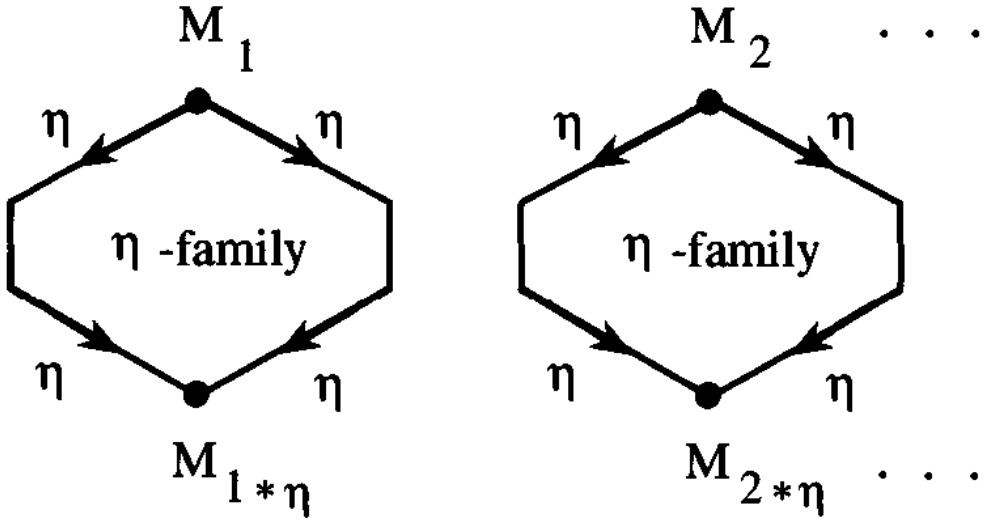
\includegraphics[scale=0.4]{fig1.png}
   \caption{The disjoint $\eta$-families.}
   \label{fig1}
\end{figure}

\begin{lem}\label{8A10}

    \begin{itemize}


           \item[(i)] The $\eta$-families of long typed terms of type
             $\tau$ partition $Nhabs(\tau)$ into non-overlapping
             finite subsets, each $\eta$-family contain one long
             member and one $\beta \eta$-nf.

         \item[(ii)] $\#(\tau)$ is infinte, finite or zero according
           to $\#_\eta(\tau)$ is infinite, finite or zero.

        \item[(iii)] $\#_{\eta}(\tau) = \#(Long(\tau))$

      \end{itemize}
\end{lem}

\begin{proof}
The following itens summarize the demostration:
 \begin{itemize}
  \item $M^{\tau} \in \mathbb{TT}(\Gamma), \,\,\,\{M^{\tau}\}_{\eta}$ is finite (by the lemma \textbf{CR}$_{\eta}$); 
  \item $\{M^{\tau}\}_{\eta} \subseteq \mathbb{TT}(\Gamma)$ (lemma \textbf{5B7.1});
  \item if $M^{\tau}$ is a $\beta$-nf then so are all members of $\{M^{\tau}\}$ (typed analogue of the lemma \textbf{1C9.3});
 \begin{center}
  $M^{\tau} \in Nhabs(\tau) \,\,\,\Longrightarrow \,\,\,\{M^{\tau}\}_{\eta} \subseteq Nhabs(\tau)$;
 \end{center}
  \item if $M^{\tau}$ is a $\beta$-nf its $\eta$-family contains exactly one $\beta\eta$-nf (typed analogue of the lemma \textbf{1C9.3});
  \item each normal inhabitant of $\tau$ is in the $\eta$-family of exactly one long normal inhabitant (by the lemma \ref{8A8});
  \item And by the \textbf{WN} lemma, $\#(\tau)$ is infinte, finite or zero according to  $\#_\eta(\tau)$ is infinite, finite or zero.
 \end{itemize}
\end{proof}


\begin{mydef}[Principal Inhabitants]

An untyped term $M$ of type $\tau$ is called principal iff $\tau$ is
the principal type of $M$. The inhabitant $M^{\tau}$ of $\tau$ is
called principal iff the deduction of $\mapsto M^{\cancel{\tau}} :
\tau$ is principal.

The set of principal inhabitants of $\tau$ is

   \begin{center}
         $Princ(\tau)$
   \end{center}

And the set of principal inhabitants in $\beta$-nf of $\tau$ is

   \begin{center}
      $Nprinc(\tau)$
    \end{center}
\end{mydef}

\begin{lem}

  $M^{\tau}$ is a principal $\beta$-nf inhabitant of $\tau$ iff $M$ is an untyped
  $\beta$-nf inhabitant of $\tau$.

\end{lem}

\begin{proof}
By the lemma \textbf{5B7.1(b)} $M^{\tau}$ is a $\beta$-nf iff $M^{\cancel{\tau}}$ is a $\beta$-nf. And, by the 
theorem \textbf{5A7}, $\tau$ is a principal type of $M$ iff $M^{\tau}$ has $\tau$ as principal type to.
\end{proof}

\begin{lem}
    Let $M^{\tau+}$ be the unique member of $Long(\tau)$ to which
    $M^{\tau}$ $\eta$-expands. Then

  \begin{center}
       $M^{\tau} \in Nprinc(\tau) \Longrightarrow M^{\tau+} \in Nprinc(\tau)$
   \end{center}
\end{lem}

\begin{proof}
 The $\eta$-expansion in the lemma \ref{8A8} preserves principality so the types of $z_1, ..., z_k$ are determined by the type $\tau$ of the component that is replaced.
\end{proof}

Now follow some examples of the relation between the classes of inhabitants:

\begin{figure}[h]
   \centering
   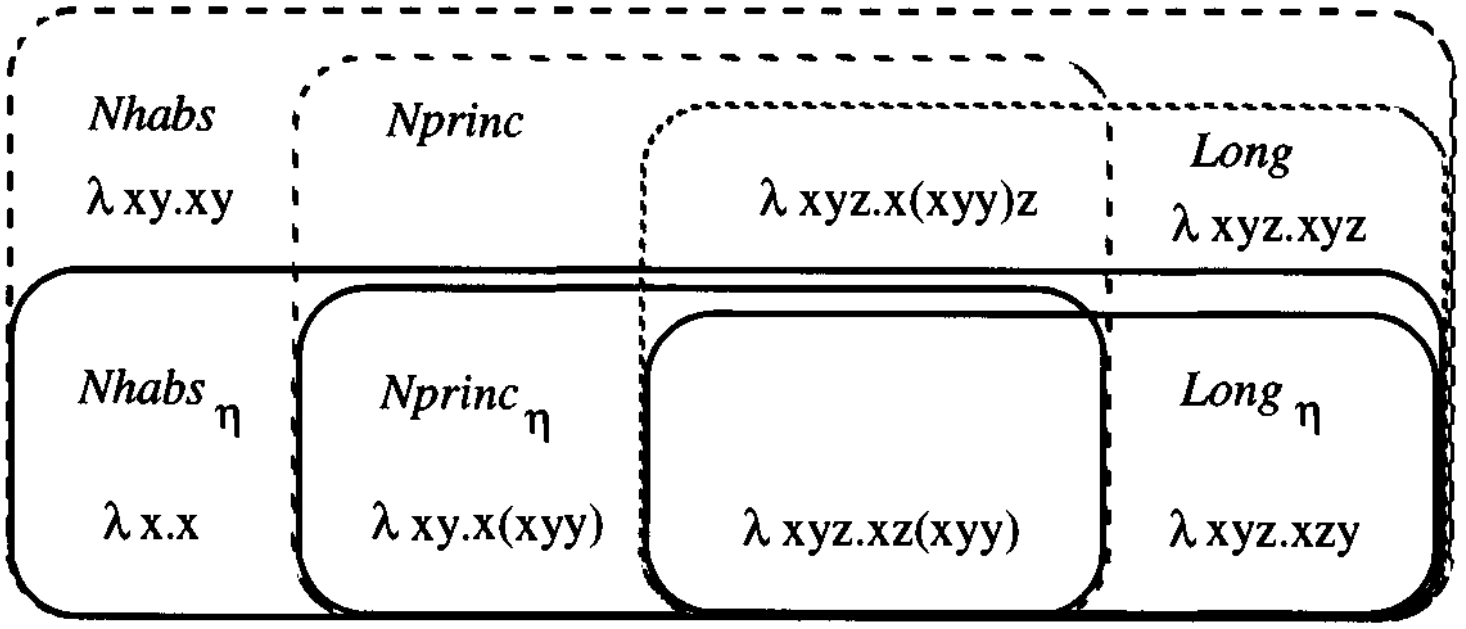
\includegraphics[scale=0.4]{fig2.png}
\end{figure}


\begin{center}
$\tau \equiv (a\to a\to a)\to a \to a \to a$\\[0.5cm]

$
\begin{array}{rlcl}
\mbox{(i)} & \lambda x^{a\to a \to a} \cdot x^{a\to a \to a} & \in & Nhabs_{\eta} - (Nprinc \cup Long)\\ 
\mbox{(ii)} & \lambda x^{a\to a \to a} \, y^{a} \cdot (x\,y)^{a \to a}& \in & Nhabs - Nhabs_{\eta} - (Nprinc \cup Long)\\ 
\mbox{(iii)} & \lambda x^{a\to a \to a} \, y^{a} \, z^{a} \cdot (x\,y\,z)^{a}& \in & Long - Nhabs_{\eta} - Nprinc\\
\mbox{(iv)} & \lambda x^{a\to a \to a} \, y^{a} \cdot (x\,(x\,y\,y))^{a \to a}& \in & Nhabs_{\eta} - Long_{\eta} \\ 
\mbox{(v)} & \lambda x^{a\to a \to a} \, y^{a} \, z^{a} \cdot (x\,(x\,y\,y)\,z)^{a}& \in & Nprinc \cap Long - Nhabs_{\eta} \\ 
\mbox{(vi)} & \lambda x^{a\to a \to a} \, y^{a} \, z^{a} \cdot (x\,z\,(x\,y\,y))^{a}& \in & Nprinc_{\eta} \cap  Long_{\eta}\\ 
\mbox{(vii)} & \lambda x^{a\to a \to a} \, y^{a} \, z^{a} \cdot (x\,z\,y)^{a}& \in &  Long_{\eta} - Nprinc_{\eta}\\ 
\end{array}
$
\end{center}

Follow the justifications:

\begin{itemize}
 \item [(i)] The term shown in (i) is clearly a $\beta\eta$-nf and is not long. It fails
to encode a principal deduction for $\lambda x\cdot x$ because the \textbf{PT} ($\lambda x\cdot x$) is not $\tau$ but $a\to a$.
 \item [(ii)] This term is obtained by $\eta$-expanding the term in (i).
 \item [(iii)] This term is obtained by $\eta$-expanding (i) until it becomes long.
 \item [(iv)] This term is easily shown to be principal by the \textbf{PT algorithm} (\textbf{3E1}). It fails
to be long because its second $x$ from the right has only one argument.
 \item [(v)] This term is obtained from (iv) by $\eta$-expansion; both occurrences of $x$ now
have two arguments.
 \item [(vi)] This term is like (v) but $z$ and $xyy$ have been reversed to make it an $\eta$-nf.
 \item [(vii)] This term is clearly long. However, its \textbf{PT} is not $\tau$ but
 \begin{center}
  $(a\to b\to c)\to b\to a\to c$
 \end{center}
\end{itemize}

\begin{remark}\label{8A13} Some remarks are important:

 \begin{itemize}
  \item [(i)] $Habs(\tau) \neq \emptyset \Longleftrightarrow Nhabs(\tau) \neq \emptyset\,\,\,\,\,$ [\textbf{WN}]
  \item [(ii)] $Habs(\tau) \neq \emptyset \Longleftrightarrow Princ(\tau) \neq \emptyset\,\,\,\,\,\,\,$ [\textbf{converse PT}]
  \item [(iii)] $Habs(\tau) \neq \emptyset \,\,\,\nRightarrow \,\,\,Nprinc(\tau) \neq \emptyset$
  \item [(iv)] $Princ(\tau) \neq \emptyset \,\,\,\nRightarrow \,\,\, Nprinc(\tau) \neq \emptyset$
 \end{itemize}
\end{remark}

The justifications for (iii) and (iv) will be given by the following note and example.
 
\begin{note}
 $\tau$ may have an inhabitant $M$, even a principal one, such that $PT(M)$ changes when $M$ is reduced to $M*_{\beta}$. 
\end{note}

\begin{exa}[$\tau \equiv a \to a \to a$] We have:
\begin{itemize}
 \item $Nhabs(\tau) = \{\lambda xy \cdot x, \lambda xy \cdot y\}$, but neither of these is principal;
 \item But there is a non-normal principal inhabitant: $(\lambda xyz \cdot \mbox{\textbf{K}}(xy)(xz))$\textbf{I}.
\end{itemize}
\end{exa}

\section{Search strategies}

The search algorithm will seek for normal long inhabitants of $\tau$ increasing a given parameter called \textbf{depth}.  
Follow some definitions, components and some informal examples of such algorithm in action.


\begin{lem}
   Every type $\tau$ has the form:

   \begin{center}
         $\tau \equiv \tau_1 \rightarrow \cdots \rightarrow \tau_m \rightarrow e$
   \end{center}
   where $m \geq 0$ and $e$ is an atomic type.
\end{lem}

\begin{proof}(Induction in $\tau$ size)\\

 \begin{itemize}
  \item if $\tau \equiv a$ then $m = 0$;
  \item if $\tau \equiv \sigma \to \rho$, by IH 
   $\sigma \equiv \sigma_1 \to \cdots \to \sigma_n \to e_{\sigma}$ and
   $\rho \equiv \rho_1 \to \cdots \to \rho_k \to e_{\rho}$, and then $m = n + k + 1$
   \begin{center}
   $\tau \equiv (\sigma_1 \to \cdots \to \sigma_n \to e_{\sigma}) \to \rho_1 \to \cdots \to \rho_k \to e_{\rho}$
   \end{center}
   
 \end{itemize}

\end{proof}


\begin{mydef}For $\tau \equiv \tau_1 \rightarrow \cdots \rightarrow \tau_m \rightarrow e$, the following definitions are convenient:
\begin{itemize}
 \item[(i)] The occurrences of $\tau_1,...,\tau_n$ and $e$ will be called \textbf{premises} and \textbf{conclusion} (or \textbf{tail}) of $\tau$;
 \item[(ii)] $m$ will be called the \textbf{arity} of $\tau$;
 \item[(iii)] Two type-occurrences will be called \textbf{isomorphic} iff they are occurrences of the same type;
 \item[(iv)] If the tail-components of $\sigma$ and $\tau$ are isomorphic we may say:
\begin{center}
 $Tail(\sigma) \cong Tail(\tau)$ 
\end{center}
\end{itemize}
\end{mydef}

\vspace*{0.5cm}

If we have that a $\beta$-nf is long, some interesting things happens with indexes in the form given in the lemma \ref{8A5}.

\begin{com}
 Let $\tau$ be any type; say $\tau$ has form
\begin{center}
 $\tau \equiv \tau_1 \rightarrow \cdots \rightarrow \tau_m \rightarrow e \,\,\,\,\,\,\, (m \geq 0, e \mbox{ an atom})$
\end{center}
and let $M^{\tau}$ be any $\beta$-nf with type $\tau$. By the lemma \ref{8A5}, $M^{\tau}$ has form
\begin{center}
 $\lambda x_1^{\tau_1} ... \,x_k^{\tau_k} \, . \,
   (v^{(\rho_1 \rightarrow \cdots \rho_n \rightarrow \tau^*)} M^{\rho_1}_1 \cdots
   M^{\rho_n}_n)^{\tau^*})^{(\tau_1 \rightarrow \cdots \tau_k \rightarrow \tau^*)}$
\end{center}
where $0 \leq k \leq m$ and $\tau^* \equiv \tau_{k+1} \to \cdots \to \tau_m \to e$.\\[0.3 cm]
If $M^{\tau} \in Long(\tau)$, then
\begin{itemize}
 \item[(i)] $k = m$ and $\tau^* \equiv e$
 \item[(ii)] the types of $x_1,..,x_m$ coincide with the premises of $\tau$
 \item[(iii)] the tail of the type of $v$ is isomorphic to $Tail(\tau)$
 \item[(iv)] if $M^{\tau}$ is closed then $m \geq 1$ and $v$ is an $x_i \,\,\, (1 \leq i \leq m)$ and
 \begin{center}
  $\tau_i \equiv \rho_1 \to \cdots \to \rho_n \to e$
 \end{center}
\end{itemize}
\end{com}


\begin{exa}[A type $\tau$ with $\#(\tau) =1$]
$\tau \equiv (a \rightarrow b \rightarrow c) \rightarrow (a\rightarrow b) \rightarrow c$ has exactly one normal inhabitant:
\begin{center}
\textbf{S}$^{\tau} \equiv \lambda x^{a \to b \to c}\,y^{a \to b}\,z^a\cdot x\,z\,(y\,z)$
is its normal inhabitant and is $\in Long(\tau) \cap Princ(\tau)$
\end{center}
\begin{proof} Follow the steps of application of the algorithm:
 \begin{itemize}
  \item[Step 1.] Start by proving that $Long(\tau) = \{\mbox{\textbf{S}}^{\tau}\}$, and looking at the structure of $\tau$; 
  by following the previous comments; we must have:\\[0.2 cm] 
  
			      $\left\{\begin{array}{lcl}
                               m & = & 3 \\
                               e & \equiv & c \\
                               \tau_1 & \equiv & a \to b \to c \\
                               \tau_2 & \equiv & a \to b \\
                               \tau_3 & \equiv & a
                              \end{array}\right.$
\vspace*{0.5 cm}
                              
So the searched term is                              
\begin{center}
$M^{\tau} \equiv (\lambda x_1^{\tau_1}\,x_2^{\tau_2}\,x_3^{\tau_3}\cdot(v^{(\rho_1 \to \cdots \rho_n \to c)}\,M_1^{\rho_1}\cdots M_n^{\rho_n})^c)^{(\tau_1 \to \tau_2 \to \tau_3 \to c)} $ 
$\in Long(\tau)$ 
\end{center}

By the item (iv) of the previous comments, $v$ must be one of $x_1, x_2, x_3$ whose type's tail is isomorphic to $Tail(\tau) \equiv c$. 
Then the unique possibly choose is $v \equiv x_1$ followed by exactly two arguments. Hence $M$ must have the form:

\begin{equation}
M \equiv \lambda x_1^{a\to b\to c}\,x_2^{a\to b}\,x_3^a \cdot x_1^{a \to b \to c}\,U^a\,V^b
\end{equation}

 \item[Step 2.] Searching for suitables $U^a$ and $V^b$ we have, by the comments(i), that $U^a \equiv (w\,P_1 \cdots P_r)^a \,\,\, (r \geq 0)$.
  And $w$ is an $x_i$ whose type's tail is isomorphic to the tail of the type of $U^a$.
  This tail is an occurrence of $a$, so $w \equiv x_3$ since $x_3$ has no premises so $r = 0$ and
\begin{equation}
 U^a \equiv x_3^a
\end{equation}
Because $b$ is an atom, $V^b$ cannot be an abstracted. Moreover its head must be $x_i$ whose type's tail is an occurrence of $b$ and
the only possibility is $x_2$, so 
\begin{equation}
  V^b \equiv x_2^{a \to b} \, W^a
\end{equation}
  \end{itemize}
 \item[Step 3.] Just as for $U^a$, the only possibility for $W^a$ is
\begin{equation}
  W^a \equiv x_3^a
\end{equation}

\noindent And now we have the conclusion (modulo $\equiv_{\alpha}$):

\begin{center}
   \textbf{S}$^{\tau} \equiv \lambda x_1^{a \to b \to c}\,x_2^{a \to b}\,x_3^a\cdot x_1\,x_3\,(x_2\,x_3) \in Long(\tau)$
\end{center}

\noindent By the lemma \ref{8A10} and the fact that \textbf{S}$^{\tau}$ is a $\beta\eta$-nf: $Nhabs(\tau) = \{S^{\tau}\}$ and, by the \textbf{PT algorithm} 
$\tau$ is a principal type of \textbf{S}$^{\tau}$: $Nprinc(\tau) = \{S^{\tau}\}$ 
\end{proof}
\end{exa}

\vspace*{0.5 cm}

\begin{exa}[A type $\tau$ with $\#(\tau) =0$] \label{8B5}
     No type that is a skeleton has inhabitants.
\begin{proof}
 Let $\tau \equiv \tau_1 \to ... \to \tau_m \to e\,\,\,(m \geq 1)$ be a skeleton. If $\tau$ had inhabitants it would have at least one long normal one, by the lemma \ref{8A8},
 and this inhabitant has the form
 \begin{center}
    $\lambda x_1\,...\,x_m\cdot x_i\,M_1\cdots M_n$
 \end{center}
There is an $x_i$ whose type is an occurrence of $e$, but $\tau$ is skeletal so $e$ cannot occur in any $\tau_i$. Hence $\tau$ has no inhabitants.
\end{proof}
\end{exa}

\vspace*{0.5 cm}

\begin{exa}[Pierce`s Law]
$\tau \equiv ((a \rightarrow b) \rightarrow a) \rightarrow a$ has no inhabitant.
\begin{proof}
  If $M^{\tau} \in Long(\tau)$ then 
  \begin{center}
       $M^{\tau} \equiv \lambda x^{(a\to b) \to a} \cdot v\,U_1\cdots U_n\,\,\,\,\,(n \geq 0)$
  \end{center}
with $v \equiv x$, since $M^{\tau}$ is closed. Hence $n = 1$
   \begin{center}
       $M^{\tau} \equiv \lambda x^{(a\to b) \to a} \cdot x^{(a\to b) \to a}\,U^{a\to b}$ 
   \end{center}
Since $a\to b$ has just one premise:
   \begin{center}
    $U^{a\to b} \equiv \lambda y^a \cdot (w\,V_1\cdots V_r)^b\,\,\,\,\, (r \geq 0)$
   \end{center}
And $M^{\tau}$ is closed so $w$ must be $x$ or $y$, at the same that it has 
a type whose tail is an occurrence of $b$, but neither $x$ nor $y$ has such type ($Long(\tau) = \emptyset$). Then we 
conclude, by the remarks and the lemma \ref{8A8} that
    \begin{center}\
    $Long(\tau) = \emptyset \Rightarrow Nhabs(\tau) = \emptyset \Rightarrow Habs(\tau) =\emptyset$
    \end{center}
\end{proof}
\end{exa}

\begin{exa}[A type $\tau$ with $\#(\tau) = m$]\label{8B4}
For $m \in \mathbb{N}^*$,  $\tau \equiv a \rightarrow \cdots \rightarrow a\,\,\,\,(m + 1\,\,a\mbox{'s})$ has $m$ inhabitants.
\begin{proof}
 Any $M^{\tau} \in Long(\tau)$ must have form
 \begin{center}
  $M^\tau \equiv \lambda x_1^a\,...\, x_m^a \cdot v\,V1 \cdots V_n$
 \end{center}
$v \equiv x_i$ for some $i\leq m$, but the types of $x_1, ..., x_m$ have no premises, so $n = 0$. Hence 
\begin{center}
 $M^{\tau} \equiv \lambda x_1^a\,...\,x_m^a \cdot x_i^a$,
\end{center}
this kind of term is called \textbf{selector} or \textbf{projector} and
\begin{center}
 $Long(\tau) \equiv Nprinc(\tau) \equiv \{\lambda x_1^a\,...\,x_m^a \cdot x_i^a\,\,|\,\,1\leq i\leq m\}$
\end{center}

\end{proof}

\end{exa}


\begin{exa}[Some other interesting examples]
Follow the example of the main combinators (\textbf{B}, \textbf{C}, \textbf{K}, \textbf{I}, \textbf{W} and the Church numerals $\bar{n}$):

\begin{center}
$
 \begin{array}{rlllll}\hline\hline
 & \mbox{\textbf{Type} } \tau             & Nhabs(\tau)         & Long(\tau)        & Nprinc(\tau)       \\\hline
 (i) & a\to a                                 & \mbox{\textbf{I}}   & \mbox{\textbf{I}} & \mbox{\textbf{I}} \\
 (ii) & a\to b\to a                            & \mbox{\textbf{K}}   & \mbox{\textbf{K}} & \mbox{\textbf{K}} \\
 (iii) & (a\to b)\to (c \to a) \to c \to b       & \mbox{\textbf{B}}   & \mbox{\textbf{B}} & \mbox{\textbf{B}} \\
 (iv) & (a\to b\to c)\to b\to a\to c            & \mbox{\textbf{C}}   & \mbox{\textbf{C}} & \mbox{\textbf{C}} \\
 (v) & (a\to a\to b)\to a\to b                 & \mbox{\textbf{W}}   & \mbox{\textbf{W}} & \mbox{\textbf{W}} \\
 (vi) & (a\to a) \to a \to a                    & \mbox{\textbf{I}}, \bar{0}, \bar{1}, \bar{2}, ... & \bar{0}, \bar{1}, \bar{2}, ... &\bar{2}, ... 
  \\\hline\hline
 \end{array}
$
\vspace*{0.5cm}

$
\begin{array}{lcllcl}
 \mbox{\textbf{B}} & \equiv & \lambda x y z \cdot x (y z) & \mbox{\textbf{C}} & \equiv &  \lambda x y z \cdot x z y \\
 \mbox{\textbf{K}} & \equiv & \lambda x y \cdot x &  \mbox{\textbf{I}} & \equiv & \lambda x \cdot x \\
 \mbox{\textbf{W}} & \equiv & \lambda x y \cdot x y y & \bar{n} & \equiv & \lambda x y\cdot x^n y 
\end{array}
$
\end{center}
\begin{proof} Follow the proofs
 \begin{itemize}
  \item [(i)] $M^{\tau} \equiv \lambda\, x_1^a\cdot x_1^a\,V_1\cdots V_n$, but $x_1^a$ admits no argument so $\{M^{\tau} \equiv \lambda\, x_1\cdot x_1\} \equiv Long(\tau)$\\ 
   (a particular case of the example \ref{8B4}, when $m = 1$);
  \item [(ii)] $M^{\tau} \equiv \lambda\,x_1^a\,x_2^b\,x_1^a\,V_1\cdots V_n$, but $x_1^a$ admits no argument so $\{M^{\tau} \equiv \lambda\,x_1^a\,x_2^b\,x_1^a\} \equiv Long(\tau)$;
  \item [(iii)] $M^{\tau} \equiv \lambda\,x_1^{a\to b}\,x_2^{c\to a}\,x_3^c\cdot x_1^{a\to b}\,U^a$, but $U^a \equiv x_2^{c \to a}\,V^c$ and $V^c \equiv x_3^c$,\\
                though $\{M^{\tau} \equiv   \lambda\,x_1^{a\to b}\,x_2^{c\to a}\,x_3^c\cdot x_1^{a\to b}\,(x_2^{c \to a}\,x_3^c)\} \equiv Long(\tau)$;
  \item [(iv)] $M^{\tau} \equiv \lambda\,x_1^{a\to b\to c}\,x_2^b\,x_3^a\cdot x_1\,U^a\,V^b$, but $U^a\equiv x_3^a$ and $V^b\equiv x_2^b$,\\
                though $\{M^{\tau} \equiv \lambda\,x_1^{a\to b\to c}\,x_2^b\,x_3^a\cdot x_1^{a\to b\to c}\,x_3^a\,x_2^b\} \equiv Long(\tau)$;
  \item [(v)] $M^{\tau} \equiv \lambda\,x_1^{a\to a\to b}\,x_2^a\cdot x_1^{a\to a\to b}\,U^a\,V^a$, but $U^a \equiv V^a \equiv x_2$,\\
		though $\{M^{\tau} \equiv \lambda\,x_1^{a\to a\to b}\,x_2^a\cdot x_1^{a\to a\to b}\,x_2^a\,x_2^a\} \equiv Long(\tau)$;
  \item [(vi)] $M^{\tau} \equiv \lambda\,x_1^{a\to a}\,x_2^a\cdot x_1^{a\to a}\,V_1^a$ or $M^{\tau} \equiv \lambda\,x_1^{a\to a}\,x_2^a\cdot x_2^a$, 
               but $V_1^a \equiv x_1^{a\to a}\,V_2^a$ or $V_1^a \equiv x_2^a$,\\
               and this process can be done indefinitely to conclude that \\
               $Long(\tau) \equiv \{\lambda\,x_1\,x_2\cdot x_2\equiv \bar{0},\, \lambda\,x_1\,x_2\cdot x_1\,x_2\equiv \bar{1},\,\lambda\,x_1\,x_2\cdot x_1\,(x_1\,x_2) \equiv \bar{2},\, ...,\, \lambda\,x_1\,x_2\cdot x_1^n\,x_2\equiv \bar{n},\, ...\}$
 \end{itemize}
 An important observation is that in the items (i) to (v) $Nhabs(\tau) \equiv Long(\tau) \equiv Nprinc(\tau)$, but in (vi) we have a trivial inhabitant in $Nhabs(\tau) - Long(\tau)$
 not reached by the algorithm (the identity $\mbox{\textbf{I}}$). Moreover one could check in the same item (by the \textbf{PT algorithm}) that the type $\tau$ is not
 a principal type for $\bar{0}$ and $\bar{1}$ but only for $\bar{2},\,\bar{3},\,...$ . If $n \geq 2$ it forces the arguments of the principal type being an a occurrence of the type $a$. 
\end{proof}
\end{exa}


\section{The search and the counting algorithms}

Now, after a quick definitions of $\mathbb{D}(\tau)$ and $Depth(\tau)$, we are only enunciating these two lemmas (The stretching and the shrinking lemma) 
and their proofs will be given to the end of the section \ref{stretching-shrinking}.


  \begin{mydef}
        $\mathbb{D}(\tau) := |\tau| \times ||\tau||$. Where $|\tau|$ is the number of atom occurrences and $||\tau||$
        is the number of distinct atom in $\tau$.
  \end{mydef}
  
  \begin{mydef}\label{8A6}
 The depth of typed or untyped terms is given by:
 
 \begin{itemize}
     \item[(i)] $Depth(\lambda x_1\, \cdots \, x_m\, . \, y) = 0$
      \item[(ii)] $Depth(\lambda x_1\, \cdots \, x_m\, . \, y \,M_1 \cdots M_n) = 1+ \underset{1 \leq j \leq n}{Max}\,Depth(M_j)\,\,\,\,\,\,\,$ if $n > 0$
  \end{itemize}
\end{mydef}

\begin{notation} The sets of all long normal inhabitants of $\tau$ (typed or untyped) with $Depth \leq d$ will both be called $Long(\tau,d)$.  
\end{notation}

  
\begin{lem}[Stretching Lemma]\label{8D2} If $Long(\tau)$ has a member $M^{\tau}$ with depth $d \geq \rVert\tau\rVert$ then it has members depths greater than any given integer,
and hence is infinite.
\end{lem}

\begin{lem}[Shrinking Lemma]\label{8D3} If $Long(\tau)$ has a member $M^{\tau}$ with depth $\geq \mathbb{D}(\tau)$ then it has a member $N^{\tau}$ with:
\begin{center}
$\mathbb{D}(\tau) - \rVert\tau\rVert \leq Depth(N^{\tau}) < \mathbb{D}(\tau)$ 
\end{center}
\end{lem}

\begin{col}\label{8D3.1} If $Long(\tau)$ has a member $M^{\tau}$ with depth $\geq \mathbb(\tau)$ then it has a member $N^{\tau}$ with 
\begin{center}
 $\rVert\tau\rVert \leq Depth(N^{\tau}) < \mathbb{D}(\tau)$
\end{center}
\begin{proof}
If $Long(\tau)$ has a member then $\tau$ is composite by the lemma \ref{8B5}. Hence $\rvert \tau \rvert \geq 2$, so
\begin{center}
$\mathbb{D}(\tau) - \rVert\tau\rVert \geq 2 \rVert\tau\rVert - \rVert\tau\rVert = \rVert\tau\rVert$ 
\end{center}
and by the lemma \ref{8D3}
\begin{center}
$ \rVert\tau\rVert \leq \mathbb{D}(\tau) - \rVert\tau\rVert \leq Depth(N^{\tau}) < \mathbb{D}(\tau)$  
\end{center}

\end{proof}
\end{col}


\begin{lem}
$Depth(M) < |M|$
\end{lem}

\begin{proof}
  Let $M \equiv \lambda x_1\, \cdots \, x_n\, . \, y M_1 \cdots M_m$. The induction is in $m$ and in $|M|$.

\begin{itemize}
 \item[(IB)] :  $m=0$, so  $M \equiv \lambda x_1\, \cdots \, x_n\, . \, y$. 
 $Depth(\lambda x_1\, \cdots \, x_n\, . \, y) = 0 < n+1 =|\lambda x_1\, \cdots \, x_n\, . \, y|$.
 
 \item[(IH)] : By induction hypothesis:
        \begin{itemize}
         \item $Depth(\lambda x_1\, \cdots \, x_n\, . \, y M_1 \cdots M_k) = 1+ Max\{Depth(M_j) \,|\,1 \leq j \leq k\} < \,|\,\lambda x_1\, \cdots \, x_n\, . \, y M_1 \cdots M_k|$;
         \item $Depth(M_{k+1}) < |M_{k+1}|$.
        \end{itemize}

But, \begin{itemize}
       \item $Depth(\lambda x_1\, \cdots \, x_n\, . \, y M_1 \cdots M_{k+1}) = 1+ Max\{Depth(M_j)\,|\,1 \leq j \leq k+1\}$ and
       \item $1+ Max\{Depth(M_j)\,|\,1 \leq j \leq k+1\} < |\lambda x_1\, \cdots \, x_n\, . \, y M_1\cdots M_k| + |M_{k+1}|$ and
       \item $|\lambda x_1\, \cdots \, x_n\, . \, y M_1\cdots M_k| + |M_{k+1}| = |\lambda x_1\, \cdots \, x_n\, . \, y M_1 \cdots M_k M_{k+1}|$
     \end{itemize}
     

Thus, 

$Depth(\lambda x_1\, \cdots \, x_n\, . \, y M_1 \cdots M_{k+1})  < |\lambda x_1\, \cdots \, x_n\, . \, y M_1 \cdots M_k M_{k+1}|$.    
        
\end{itemize}
\end{proof}


\begin{mydef}[nf-schemes]\label{8C1}
 A \textbf{nf-scheme} is a $\beta$-nf that may contain meta-variables under restrictions:
 \begin{itemize}
  \item[(i)] each nf-scheme is a $\beta$-nf without bound-variables clashes;
  \item[(ii)] meta-variables do not bind ($\lambda V$ is forbidden);
  \item[(iii)] in a composite nf-scheme meta-variables only occur in argument positions;
  \item[(iv)] each meta-variable in a nf-scheme occurs only once.
 \end{itemize}
\end{mydef}

\begin{mydef}[Proper nf-scheme]\label{8C1.1}
 A \textbf{proper nf-scheme} is a nf-scheme that contain at least one meta-variable.
\end{mydef}


\begin{lem}[Search Theorem for $Long(\tau)$]\label{8C5}
  The search algorithm below accepts any composite type $\tau$ and
  outputs a finite or infinite sequence of sets $\mathcal{A}(\tau,d) (d =
  0,1,2,3,\cdots)$,

    \begin{itemize}
           \item[(i)] each member of $\mathcal{A}(\tau,d)$ is a closed long
             typed nf-scheme with type $\tau$, and is either

             \begin{itemize}
                   \item a proper nf-scheme with depth $d$, or
                   \item a term with depth $d-1$
             \end{itemize}

             \item[(ii)] $\mathcal{A}(\tau,d)$ is finite.

             \item[(iii)] $Long(\tau,d) \subseteq \mathcal{A}(\tau,0) \cup
               \cdots \cup \mathcal{A}(\tau,d)$

             \item[(iv)] If the set of all terms in $\mathcal{A}(\tau,d)$ is
               called $\mathcal{A}_{terms}(\tau,d)$, then :

               \begin{center}
                     $Long(\tau) = \bigcup_{d \geq 0}\mathcal{A}_{terms}(\tau,d)$
               \end{center}
    \end{itemize}
\end{lem}

\begin{proof}

  The proof of {\em (i)} and {\em (ii)} is using induction in $d$.

  \begin{itemize}
          \item[(IB)] The induction base : if $d=0$, then $\mathcal{A}(\tau,d) =
            {V^{\tau}}$ or $\mathcal{A}(\tau,d) =
            \emptyset$. In any way, each element of
            $\mathcal{A}(\tau,d)$ has depth $0$ and the set is finite.

            \item[(IH)] Assume, by induction hypothesis, that for all
              $k$ less or equal than $d$ : 
              \begin{itemize}
                     \item[(i)] $\mathcal{A}(\tau,k)$ is finite 
                     \item[(ii)] each member of $\mathcal{A}(\tau,k)$ is a closed long
                     \item[(iii)]each member of $\mathcal{A}(\tau,k)$ is a proper nf-scheme with depth $k$ or a term with depth $k-1$
             \end{itemize}

             The goal is proof that the same properties hold for
             $\mathcal{A}(\tau,d+1)$. In other to do it, it will be
             analyzed each case of algorithm in the computation of $\mathcal{A}(\tau,d+1)$.

             \item[(Case 1)] $\mathcal{A}(\tau,d) = \emptyset$ or no
               member of $\mathcal{A}(\tau,d)$ contains a  meta-variable.

               If $\mathcal{A}(\tau,d) = \emptyset$, then, by vacuity, the
               properties hold.

               If no member of $\mathcal{A}(\tau,d)$ contains a
               meta-variable, the answer is the sequence
               $\mathcal{A}(\tau,0), \cdots ,\mathcal{A}(\tau,d)$,
               however, the answer is undefined.

               \item[(Case 2)] Take one member of
                 $\mathcal{A}(\tau,d)$. By IH, it is a proper
                 nf-scheme with depth $d$ or a term with depth
                 $d-1$. Suppose that this member is a proper
                 nf-scheme. Any suitable replacement of it has the form $\lambda
                 x_1 \cdots x_n \cdot(h V_1 \cdots V_m)$. If $m=0$ for
                 all of that, they must have the form $\lambda
                 x_1 \cdots x_n \cdot h$ and the result is a closed
                 lambda term. The depth of all suitable replacement
                 is $0$ and the depth of the closed lambda, that belongs to $\mathcal{A}(\tau,d+1)$, term is
                 $d$. In the other hand, if $m > 0$, the depth of $\lambda
                 x_1 \cdots x_n \cdot(h V_1 \cdots V_m)$ is 1. Thus, after all the replacements of the meta-variables, the depth of the proper nf-scheme increases 1. Therefore, the result is a nf-scheme with depth $d+1$, that belongs to $\mathcal{A}(\tau,d+1)$. The number of replacements is finite, thus, the number of elements in $\mathcal{A}(\tau,d+1)$ is also finite.
                 
    \end{itemize}

    The item {\em (iii)} states that the algorithm is complete and its proof is postponed to the lemma \ref{8F1}. The Part {\em (iv)} follows easily from {\em (i)-(iii)}.
\end{proof}


\begin{mydef}\label{8D1}
For the sets $\mathcal{A}(\tau,d)$ and $\mathcal{A}_{\mbox{\footnotesize terms}}(\tau,d)$, define:
 \begin{center}
 $\begin{array}{lcl}
   \mathcal{A}(\tau,\leq d) & = &  \mathcal{A}(\tau,0) \cup ... \cup \mathcal{A}(\tau,d) \\
   \mathcal{A}_{\mbox{\footnotesize terms}}(\tau,\leq d) & = &  \mathcal{A}_{\mbox{\footnotesize terms}}(\tau,0) \cup ... \cup \mathcal{A}_{\mbox{\footnotesize terms}}(\tau,d)
  \end{array}$
  \end{center}
\end{mydef}


% \begin{mydef}
%        The sets $\mathcal{A}(\tau, \leq d)$ and
%        $\mathcal{A}_{terms}(\tau, \leq d )$ are defined as:
% 
%        \begin{itemize}
%            \item[(i)] $\mathcal{A}(\tau, \leq d) = \mathcal{A}(\tau,0)
%              \cup \cdots \cup \mathcal{A}(\tau,d)$
%             \item[(ii)] $\mathcal{A}_{terms}(\tau, \leq d) = \mathcal{A}_{terms}(\tau,0)
%              \cup \cdots \cup \mathcal{A}_{terms}(\tau,d)$
%         \end{itemize}
% \end{mydef}


\begin{mydef}[The search algorithm $\mathcal{A}(\tau,n)$]\label{8C6}

input: any type $\tau$

If $\tau$ is an atom, it as no inhabitant.

Otherwise,

\begin{enumerate}
      \item Chose a meta-variable $V$ :
        \begin{center}
              $A(\tau,0) = V^{\tau}$
        \end{center}

      \item[$d+1$] Assume that $A(\tau,d)$ is defined.
        
        \begin{enumerate}
              \item If $A(\tau,d) = \emptyset$ or no member of
                $A(\tau,d)$ contains meta-variable, then
                stop. $A(\tau,d+1)$ is undefined, and the algorithm
                outputs the sequence $A(\tau,1), \cdots, A(\tau,d)$.

                \item Otherwise, apply the following steps:

                \begin{enumerate}
                       \item Given any proper $X^{\tau} \in A(\tau,d)$, list
                       the meta-variables of $X^{\tau}$:

                       \begin{center}
                              $V^{\rho_1}_1, \cdots, V^{\rho_n}_n$
                         \end{center}
                         Apply the following steps to each
                         meta-variable:

                         \begin{enumerate}
                                \item Given any meta-variable
                                  $V^{\rho}$ in $X^{\tau} \in
                                  A(\tau,d)$, say :
                                 
                                 \begin{center}
                                       $\rho \equiv \sigma_1 \rightarrow
                                       \cdots \rightarrow \sigma_m
                                       \rightarrow a$
                                 \end{center}
                                 
                                 \item List all $\sigma_j$ such that
                                   $tail(\sigma_j) \cong a \cong
                                   tail(\rho)$. Each $\sigma_j$ has
                                   the form:

                                   \begin{center}
                                         $\sigma_j \equiv \sigma_{j,1}
                                         \rightarrow \cdots
                                         \rightarrow \sigma_{j,n_j}
                                         \rightarrow a$
                                   \end{center}

                                   Thus, define:
                                   \begin{center}
                                         $Y^{\rho}_j \equiv \lambda
                                         x^{\sigma_1}_1 \cdots
                                         x^{\sigma_m}_m \cdot
                                         (x^{\sigma_j}_j
                                         V^{\sigma_{j,1}}_{j,1} \cdots
                                         V^{\sigma_{j,n_j}}_{j,n_j})^{a}$
                                   \end{center}

                                   \item List the abstractors that
                                     cover the occurrence of $V^{\rho}$
                                     in $X^{\tau}$ in order that they
                                     occur. They are:

                                     \begin{center}
                                            $\lambda z^{\zeta_1}_1 \cdots z^{\zeta_t}_t$
                                     \end{center}

                                     List each $\zeta_i$ such that
                                     $tail(\zeta_i) = a$. It has the
                                     form:

                                     \begin{center}
                                           $\zeta_i \equiv \zeta_{i,1}
                                           \rightarrow \cdots
                                           \rightarrow \zeta_{i.h_i}
                                           \rightarrow a$
                                     \end{center}

                                     Define

                                     \begin{center}
                                           $Z^{\rho}_i \equiv \lambda
                                           x^{\sigma_1}_1 \cdots
                                           x^{\sigma_m}_m \cdot
                                           (z^{\zeta_i}_i V^{\zeta_{i,1}}_{i,1} \cdots V^{\zeta_{i,h_i}}_{i,h_i})^a$
                                     \end{center}
                         \end{enumerate}

                         \item When the last step was applied in all
                           meta-variables in $X^{\tau}$, the result is
                           a list of suitable replacements of $V_i$ in
                           $X^{\tau}$. If at least one of $V_1 \cdots
                           V_q$ has no suitable replacements, abandon
                           $X^{\tau}$, call it a reject, and start
                           applying step b to the next member of
                           $A(\tau,d)$.

                           If all $V_1 \cdots V_q$ has  suitable
                           replacements, $X^{\tau}$ is called
                           extendable. In this case, list all possible
                           replacements:
                           \begin{center}
                                 $\langle W^{\rho_1}_1, \cdots,
                                 W^{\rho_q}_q \rangle$
                           \end{center}

                           Where each $W^{\rho_j}_j$ is a suitable
                           replacement for $V_j$. For each element of
                           sequence, construct a new nf-scheme
                           $X^{*\rho}$ from $X^{\rho}$, replacing
                           $V_j$ for $W^{\rho_j}_j$.
                \end{enumerate}

                \item If $A(\tau, d )$ contains at least one
                  nf-scheme, define $A(X^{\tau},d+1)$ contain all the
                  extensions of all extendable proper of nf-schemes in $A(\tau,d)$
        \end{enumerate}
\end{enumerate}
\end{mydef}

\begin{exa}
  Apply the search algorithm for the following type:
     \begin{center}
           $\tau \equiv (a \to b \to c)\to (a \to b) \to a \to c$
     \end{center}
     Consider $SR(V^{\sigma})$ as a list of suitable replacements of $V^{\sigma}$.
     The sets are:
     \begin{center}
          $\mathcal{A}(\tau,0) = \{ V^{\tau}_1\}$
     \end{center}

     \begin{center}
          $SR(V^{\tau}_1) = \langle \lambda x^{a\to b \to c}_1 x^{a\to b}_2
          x^{a}_3 \cdot x^{a\to b \to c}_1 V^{a}_2 V^b_3 \rangle$
     \end{center}

     \begin{center}
          $\mathcal{A}(\tau,1) = \{ \lambda x^{a\to b \to c}_1 x^{a\to b}_2
          x^{a}_3 \cdot x^{a\to b \to c}_1 V^{a}_2 V^b_3\}$
     \end{center}

     \begin{center}
            $SR(V^{a}_2 ) = \langle x^{a}_3 \rangle$
     \end{center}
     

     \begin{center}
          $SR(V^b_3  ) = \langle x^{a\to b}_2 V^{a}_4\rangle$
     \end{center}

     \begin{center}
          $\mathcal{A}(\tau,2) = \{ \lambda x^{a\to b \to c}_1 x^{a\to b}_2
          x^{a}_3 \cdot x^{a\to b \to c}_1 x^{a}_3 x^{a\to b}_2 V^{a}_4\}$
     \end{center}

     \begin{center}
            $SR(V^{a}_4 ) = \langle x^{a}_3 \rangle$
     \end{center}

     \begin{center}
          $\mathcal{A}(\tau,3) = \{ \lambda x^{a\to b \to c}_1 x^{a\to b}_2
          x^{a}_3 \cdot x^{a\to b \to c}_1 x^{a}_3 x^{a\to b}_2 x^{a}_3\}$
     \end{center}
\end{exa}

\begin{exa}
       Apply the search algorithm for the following type:
     \begin{center}
           $\tau \equiv a \to \cdots \to a \to a$
     \end{center}

     Where $|\tau| = m+1$. The sets are:
     \begin{center}
          $\mathcal{A}(\tau,0) = \{ V^{\tau}_1\}$
     \end{center}

     \begin{center}
          $SR(V^{\tau}_1) = \langle (\lambda x^{a}_1 \cdots
          x^{a}_{m+1} \cdot x^{a}_1), \cdots, (\lambda x^{a}_1 \cdots
          x^{a}_{m+1} \cdot x^{a}_{m+1}) \rangle$
     \end{center}

     \begin{center}
              $\mathcal{A}(\tau,1) = \{ (\lambda x^{a}_1 \cdots
          x^{a}_{m+1} \cdot x^{a}_1), \cdots, (\lambda x^{a}_1 \cdots
          x^{a}_{m+1} \cdot x^{a}_{m+1}) \}$
     \end{center}
\end{exa}

\begin{exa}
  Apply the search algorithm for the following type:
     \begin{center}
           $\tau \equiv ((a \to b) \to a) \to a$
     \end{center}

     The sets are:
     \begin{center}
          $\mathcal{A}(\tau,0) = \{ V^{\tau}_1\}$
     \end{center}

     \begin{center}
            $SR(V^{\tau}_1 ) = \langle \lambda x^{(a \to b) \to a}_1. V^{a}_2 \rangle$
     \end{center}

     \begin{center}
            $\mathcal{A}(\tau,1) = \{ \lambda x^{(a \to b) \to a}_1. V^{a}_2 \}$
     \end{center}

     \begin{center}
            $SR(V^{a}_2  ) = \langle x^{(a \to b) \to a}_1 V^{a \to b}_3 \rangle$
     \end{center}

     \begin{center}
            $\mathcal{A}(\tau,2) = \{ \lambda x^{(a \to b) \to
              a}_1. x^{(a \to b) \to a}_1 V^{a \to b}_3 \}$
     \end{center}

     \begin{center}
            $SR(V^{a \to b}_3  ) = \langle \rangle$
     \end{center}

     \begin{center}
            $\mathcal{A}(\tau,3) = \emptyset$
     \end{center}
\end{exa}

\begin{mydef}[Counting Algorithm for $Long(\tau)$]\label{8D5} In $\tau$ is an atom, $Long(\tau)$ is empty by the lemma \ref{8B5}. If $\tau$ is
composite, apply the search algorithm (definition \ref{8C6}) to $\tau$; this outputs a finite or infinite sequence of sets
\begin{center}
 $\mathcal{A}(\tau,d) \,\,\,\,\, (d = 0, 1, 2, ...)$
\end{center}

Stop the search algorithm at $d = \mathbb{D}(\tau)$ and enumerate $\mathcal{A}_{\mbox{\footnotesize terms}}(\tau, \leq \mathbb{D}(\tau))$.\\

\noindent{\em [By the lemma \ref{8C5}, if $Long(\tau)$ had a member with depth $\geq \mathbb{D}(\tau)$\\ 
it would have one with depth $< \mathbb{D}(\tau)$.]}\\

\begin{itemize}
 \item[{\em \textbf{Case I}:}] $\mathcal{A}_{\mbox{\footnotesize terms}}(\tau, \leq \mathbb{D}(\tau)) = \emptyset$.\\
 
{\em [By the lemma \ref{8D3}, if $Long(\tau)$ had a member with depth $\geq \mathbb{D}(\tau)$\\ 
it would have one with depth $< \mathcal{D}(\tau)$.]} 
 
 \item[{\em \textbf{Case II}:}] $\mathcal{A}_{\mbox{\footnotesize terms}}(\tau, \leq \mathbb{D}(\tau))$ has a member with depth $\geq \rVert\tau\rVert$.
 Then by the lemma \ref{8D2} $Long(\tau)$ is infinite. To enumerate $Long(\tau)$, apply the search algorithm to enumerate $\mathcal{A}_{\mbox{\footnotesize terms}}(\tau, d)$\\
 for $d = 0, 1, 2, ..$.

 {\em [By the lemma \ref{8C5}(iv) the union of these sets is $Long(\tau)$].}
 
 \item[{\em \textbf{Case III}:}] $\mathcal{A}_{\mbox{\footnotesize terms}}(\tau, \leq \mathbb{D}(\tau))$ has members but they all have depth $< \rVert\tau\rVert$. 
 Then $Long(\tau) = \mathcal{A}_{\mbox{\footnotesize terms}}(\tau, \leq \mathbb{D}(\tau))$, which is finite.\\
 
{\em [The only way for $Long(\tau)$ to differ from this set would be for $Long(\tau)$ to \\
 have members with depth $d \geq \mathbb{D}(\tau))$, but by the lemma \ref{8D3.1} it would then have a member\\ 
 with $\rVert\tau\rVert \leq d < \mathbb{D}(\tau))$ contrary to the assumption of the present case.]}
 
\end{itemize}
\end{mydef}


\begin{theo}[Counting long normal inhabitants]\label{8D4}When given a type $\tau$ the Counting Algorithm outputs $\# \mbox{Long}(\tau)$ and an enumeration 
 of $Long(\tau)$.
\begin{proof}
 The proof is in the above brackets with the algorithm's description. 
\end{proof}
\end{theo}

\begin{col}[Counting $\beta\eta$-normal inhabitants]\label{8D5.1}The algorithm of the definition \ref{8D5} can be used to count and enumerate
$Nhabs_{\eta}(\tau)$ for every $\tau$.
\begin{proof}
By \ref{8A10} the members of \textit{Nhabs}$_{\eta}(\tau)$ are the $\eta$-nf's of those $Long(\tau)$. And by the lemma \ref{8A10}(iii), 
$\#_{\eta}(\tau) = \#(Nhabs_{\eta}(\tau)) = \#(Long(\tau))$.
\end{proof}
\end{col}

\begin{col}[Emptiness test]\label{8D5.2} The algorithm of the definition \ref{8D5} can be used to decide whether a type $\tau$ has no inhabitants.
\begin{proof}
By the remark \ref{8A13}(i), $Habs(\tau) = \emptyset \Leftrightarrow \#(Nhabs(\tau)) = \#(\tau) = 0$. And by the lemma \ref{8A10}(ii) and (iii),
$\#(\tau) = 0 \Leftrightarrow \#(Long(\tau)) = 0$.
\end{proof}
\end{col}

\begin{mydef}[Counting Algorithm for $Nhabs(\tau)$]\label{8D7} If $\tau$ is an atom then $Nhabs(\tau)$ is empty by the lemma \ref{8B5}. 
If $\tau$ is composite, apply the algorithm of the definition \ref{8D5} to count $Long(\tau)$.
\begin{itemize}
 \item[\textbf{Case I}:] If $Long(\tau) = \emptyset$ then $Nhabs(\tau) = \emptyset$.\\ 
 
 {\em [By the lemma \ref{8A8}.]}
 
 \item[\textbf{Case II}:] If $Long(\tau) \neq \emptyset$ then $Nhabs(\tau)$ is counted and enumerated by counting and 
 enumerating $Long(\tau)$ and enumerating the $\eta$-family of each member of $Long(\tau)$.\\
 
 {\em [By the lemma \ref{8A10} these $\eta$-families are finite and their union is in $Nhabs(\tau)$.] }
 
\end{itemize}
\end{mydef}

\begin{theo}[Counting all normal inhabitants]\label{8D6} When given a type $\tau$ the algorithm of the definition \ref{8D7} outputs $\#(\tau)$ and an
enumeration of the set $Nhabs(\tau)$ of all $\beta$-normal inhabitants of $\tau$.
\begin{proof}
 The proof is in the above brackets with the algorithm's description. 
\end{proof}
\end{theo}

\begin{mydef}\label{8D8}
 A type $\tau$ will be called \textbf{monatomic} iff $\rVert\tau\rVert = 1$, i.e. iff only one atom occurs in $\tau$.
\end{mydef}

\begin{theo}\label{8D9} Let $\tau$ be a monatomic type with the form $\tau \equiv \tau_1 \to ... \tau_m \to a \,\, (m \geq 0)$. Then
\begin{itemize}
 \item[(i)] if at least one $\tau_i$ is composite, $\#(\tau)$ is either $\infty$ or 0;
 \item[(ii)] if $\tau_1 \equiv ... \equiv \tau_m \equiv a$ then $\#(\tau) = m$.
\end{itemize}

\begin{proof}
The part (ii) is simple application of the lemma \ref{8B4}. To prove (i), assuming that $Nhabs(\tau)$ is finite and non-empty and that
$\tau$ has form
\begin{center}
 $\tau \equiv \tau_1 \to ... \to \tau_m \to a$
\end{center}
with $m \geq 1$ and at least one premise composite. By the lemma \ref{8A8} $Long(\tau)$ is also finite and has a member $M^{\tau}$.
By the lemma \ref{8D2}, $Depth(M^{\tau}) < \rVert\tau\rVert = 1$, so $M^{\tau}$ must have form
\begin{center}
$M^{\tau} \equiv \lambda x_1^{\tau_1} ...\,x_m^{\tau_m} \cdot x_p^{\tau_p}  \,\,\,\,\,\,\, (1 \leq p \leq m).$ 
\end{center}
And $\tau_p \equiv a$ since $M^{\tau}$ is long. Choose a composite premise of $\tau$; say it is $\tau_i$ and has form
\begin{center}
$\tau_i \equiv \tau_{i,1} \to ... \to \tau_{i,m_i} \to a \,\,\,\,\,\,\,  (m_i \geq 1).$  
\end{center}
For $j = 1,...,m_i$ each $\tau_i,j$ has form
\begin{center}
$\tau_{i,j} \equiv \tau_{i,j,1} \to ... \to \tau_{i,j,m_{i,j}}\to a \,\,\,\,\,\,\, (m_{i,j} \geq 0).$
\end{center}
For each $j \leq m_i$ choose distinct new variables $y_1, ..., y_{m_{i,j}}$ and define
\begin{center}
$P_j^{\tau_{i,j}} \equiv \lambda y_1^{\tau_{i,j,1}} ...\,y_{m_{i,j}}^{\tau_{i,j,m_{i,j}}} \cdot x_p^a$ 
\end{center}
where $x^a_p$ is the rightmost variable in $M^{\tau}$ (and is therefore distinct from the $y$'s). Then define
\begin{center}
$N^{\tau} \equiv \lambda x_1^{\tau_1} ...\,x_m^{\tau_m} \cdot (x_i^{\tau_i} P_1^{\tau_{i,1}} \cdots P_{m_i}^{\tau_{i,m_i}})^a$ 
\end{center}
Clearly $N^{\tau} \in Long(\tau)$. But $Depth(N^{\tau}) \geq 1$ since $N^{\tau}$ contains $m_i \geq 1$ arguments. 
Hence $Long(\tau)$ is infinite by the lemma \ref{8D2}.
\end{proof}
\end{theo}


\section{Search-Completeness, Stretching and Shrinking lemmas}\label{stretching-shrinking}

The aim of the this section is to prove two important lemmas that will serve as a basis for the proof of completeness of search and 
counting algorithms. The key role will lay the foundation by analyzing the structure of an arbitrary long typed nfscheme, and
will be played by a slightly strengthened form of the subformula property. That property says in effect that the types of all the components
of a closed $\beta$-nf $M^{\tau}$ are subtypes of $\tau$. This implies that all the successes
produced by the search algorithm, growing deeper and deeper, have the types of
their components drawn from the same fixed finite set. This limitation is the source
of the bounds in the stretching and shrinking lemmas.

We shall need the notation for positions, components and construction-trees. In writing positions a 
sequence of $n$ $0$'s may be written as $0^n$ (with $0^0 = \emptyset)$, and similarly for $1$'s and $2$'s.
Remembering that every non-atomic nf-scheme $X$ can be expressed uniquely in the form:
\begin{center}
 $X \equiv \lambda x_1\, ...\, x_m \cdots v\,Y_1 \cdots Y_n\,\,\,\,\,\, (m + n \geq 1)$
\end{center}
where $v$ is one of $x_1, ..., x_n$ if $X$ is closed. The construction-tree of such $X$ is shown in Fig. \ref{Fig3}. The 
\textbf{head} and \textbf{arguments} of $X$ are respectively $v$ and $Y_1,\,...,\,Y_n$. We can note that the position of $Y_i$ is
\begin{center}
 $0^m\,1^{n - i}\,2\,\,\,\,\,\,\,(1\leq i\leq n)$
\end{center}

\begin{figure}[h]
   \centering
   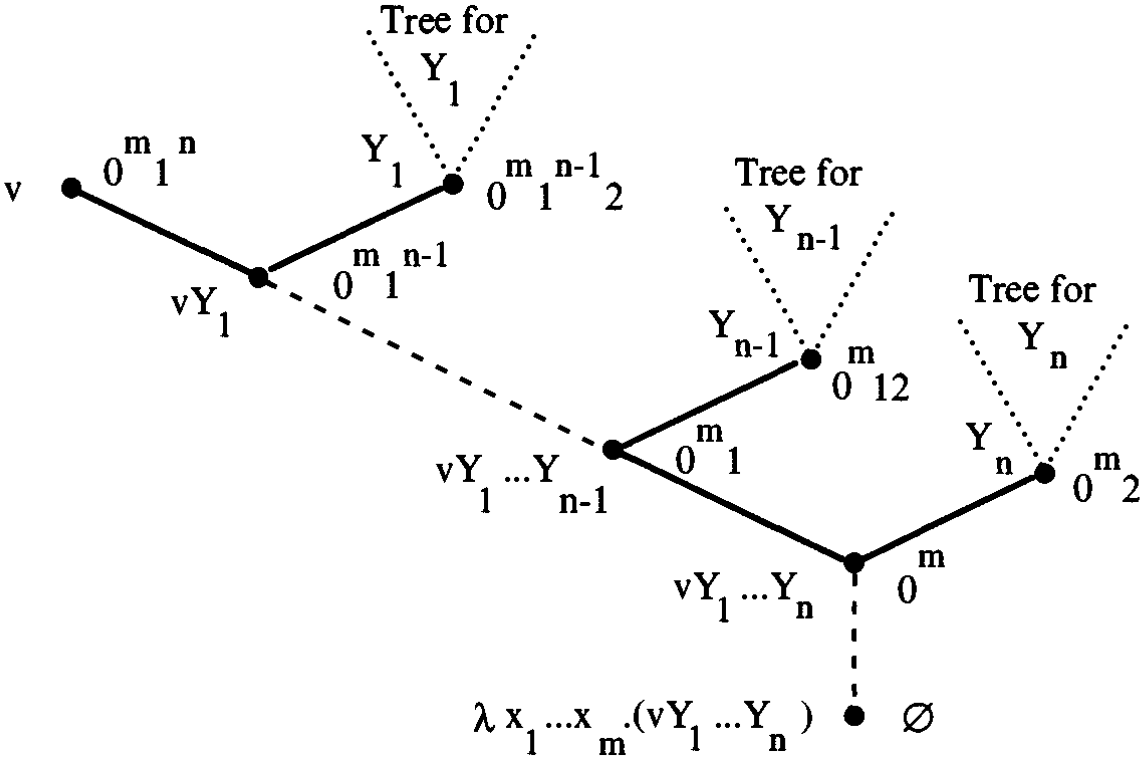
\includegraphics[scale=0.5]{fig3.png}
   \caption{The construction-tree of a nf-scheme $X$.}
   \label{Fig3}
\end{figure}

The Fig. \ref{Fig4} is presenting an example of construction tree of $\lambda x\,y\cdot x\,(\lambda u\cdot u\,V_1)\,V_2$.

\begin{figure}[h]
   \centering
   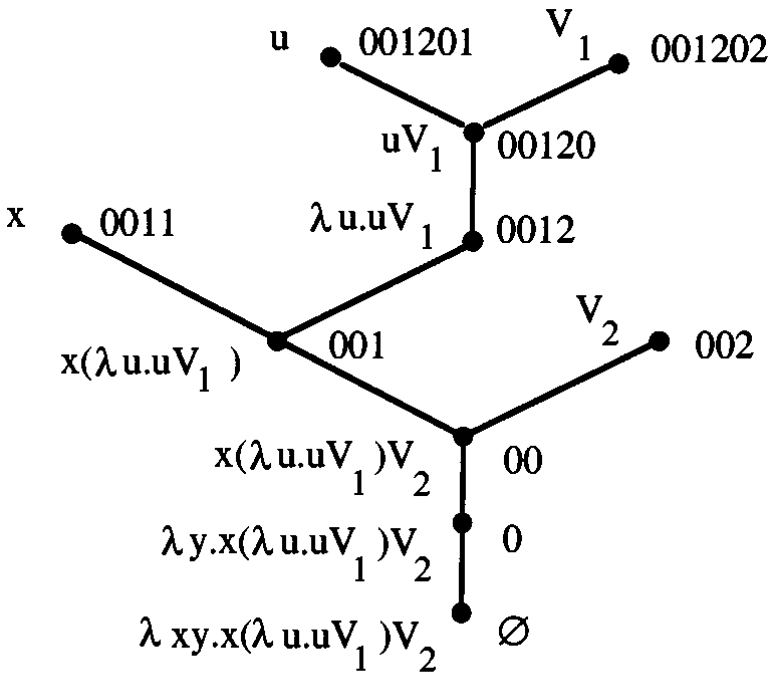
\includegraphics[scale=0.5]{fig4.png}
    \caption{The construction-tree of $\lambda x\,y\cdot x\,(\lambda u\cdot u\,V_1)\,V_2$.}
   \label{Fig4}
\end{figure}


\begin{mydef}[Typed nf-schemes, $\mathbb{TNS}(\Gamma)$]
 \textbf{Typed nf-schemes} are defined as $\mathbb{TT}(\Gamma)$ with meta-variables under the same restrictions pointed in the definition \ref{8C1}.
\end{mydef}

\begin{mydef}[Long typed nf-schemes]\label{8C4}
  A nf-scheme $X^{\tau}$ is long iff each component of $X^{\tau}$ with the form:

  \begin{center}
        $(z\,Y_1 \cdots Y_n)^{\tau}\,\,\,\,\,(n \geq 0)$
  \end{center}
   that is not in a function position has atomic type.
\end{mydef}

\begin{exa} The nf-scheme (i) below is long, though in contrast the term (ii) is not:
\begin{itemize}
 \item[(i)] $x^{(a\to b)\to c)}\,V^{a\to b}$,
 \item[(ii)] $x^{(a\to b)\to c)}\,z^{a\to b}$.
\end{itemize}
Remembering that in (i) the meta-variable $V$ could be filled with $(\lambda y^a \cdot z^b)^{a\to b}$.
\end{exa}

\begin{mydef}[Subarguments] A \textbf{subargument} of a typed or untyped nf-scheme $X$ is a component that is an
argument of $X$ or an argument of a proper component of $X$. 
\end{mydef}

\begin{note}\label{8E2.2}
 \begin{itemize} The following notes will be useful:
  \item[(i)] All occurrences of meta-variables in a composite nf-scheme are subarguments.
  \item[(ii)] A subargument of a subargument of $X$ is a subargument of $X$.
 \end{itemize}
\end{note}

\begin{lem}\label{8E2.1} A component $Y$ of a typed or untyped nf-scheme $X$ is a subargument iff its position is not $\emptyset$
and the last symbol in its position is $2$.
 \begin{proof} Induction in $|X|$:\\
 
\noindent Every non-atomic nf-scheme has the form 
  \begin{center}
   $X \equiv \lambda x_1\, ...\, x_m \cdots v\,Y_1 \cdots Y_n\,\,\,\,(n + m \geq 1)$; 
  \end{center}
   where each
   \begin{center}
    $Y_i \equiv z_i\,U_1 \cdots U_k\,\,\,\,\,(k \geq 0)$.
   \end{center}
   So following the Fig \ref{Fig3}:
   \begin{itemize} 
    \item[(IB)] If a given $Y_i$ is a meta-variable his position is $\neq \emptyset$ and it will be $0^m 1^{(n-i)} 2$;
    \item[(IS)] And if $Y_i$ is not a meta-variable, by IH, his subarguments have positions $\neq \emptyset$ and ended in $2$. 
    Then because the subarguments of $Y_i$ are subarguments of $X$ we must have that all subarguments of $X$ are 
    $\neq \emptyset$ and ended in $2$.
   \end{itemize} 
 \end{proof}
\end{lem}


\begin{mydef}[Relative depth] The $2$-\textbf{length} of a position-string $p$ is the number of $2$'s in $p$. The \textbf{depth in} $X$ of a 
subargument $Z$ of $X$ is the $2$-length of its position (i.e. the number of right-hand choices made when traveling up the tree of $X$ from
the bottom node to $Z$ (cf. Fig. \ref{Fig3})).
\end{mydef}

\begin{lem}\label{8E3.1} Let $X$ be a typed or untyped nf-scheme with $Depth(X)\geq 1$. Then
\begin{itemize}
 \item[(i)] $Depth(X)$ is the maximum of the depths in $X$ of all subarguments of $X$,
 \item[(ii)] $X$ has at least one subargument whose depth in $X$ is the same as $Depth(X)$ and each such subargument is an atom or abstract atom.
\end{itemize}
\begin{proof}(Induction in $|X|$)\\

\noindent Given $X \equiv \lambda x_1\, ...\, x_m \cdots v\,Y_1 \cdots Y_n\,\,\,\,(n + m \geq 1)$, 
  by the definition \ref{8A6} we have that:
  \begin{itemize}
   \item[(IB)] if $n = 0$ then $Depth(X) = Depth(\lambda x_1\, ...\, x_m \cdots v) = 0$ 
   \item[(IS)] if $n \neq 0$ $Depth(\lambda x_1\, ...\, x_m \cdots v\,Y_1 \cdots Y_n) = 1 + \underset{1 \leq i \leq n}{Max}\,Depth(Y_i)$
  But, by IH, for each $Y_i$ we have:
  \begin{itemize}
   \item[(i)] $Depth(Y_i)$ is the maximum of the depths in $Y_i$ of all subarguments of $Y_i$, and because of the fact that each subargument
   of $Y_i$ is a subargument of $X$, we have that {\em (i)} holds;
   \item[(ii)] each $Y_i$ has at least one subargument whose depth in $Y_i$ is the same as $Depth(Y_i)$, so by the definition of $Depth$, 
   $X$ will have at least one subargument with depth equal to $Depth(X)$.
  \end{itemize}
 \end{itemize}
 
\end{proof}
\end{lem}


\begin{mydef}[Argument-branch] If $Z$ is a subargument of a typed or untyped nf-scheme $X$, the \textbf{argument-branch from} $X$ \textbf{to} $Z$ is the 
sequence
\begin{center}
  $\langle Z_0, Z_1, ..., Z_k\rangle\,\,\,\,\,\, (k \geq 1)$
\end{center}
such that $Z_0 \equiv X$ and $Z_i$ is an argument of $Z_{i - 1}$ for $i = 1, ..., k$, and $Z_k \equiv Z$. It is called \textbf{unextendable} iff
$Z$ is an atom or abstract atom. Its \textbf{length} is $k$ (not $k + 1$).
\end{mydef}

\begin{lem}\label{8E4.1} For any typed or untyped nf-scheme $X$:
\begin{itemize}
 \item[(i)] the depth in $X$ of a subargument $Z$ is the same as the length of the argument-branch from $X$ to $Z$;
 \item[(ii)] $Depth(X)$ is the maximum of the lengths of all argument-branches in $X$.
\end{itemize}
\begin{proof} For {\em (i)} induction in $|X|$
  \begin{itemize}
   \item[(IB)] if $n = 0$ then $Depth(X) = Depth(\lambda x_1\, ...\, x_m \cdots v) = 0$ and the length to the argument-branch from $X$ to $X$ itself is $0$.
   \item[(IS)] if $n \neq 0$ $Depth(\lambda x_1\, ...\, x_m \cdots v\,Y_1 \cdots Y_n) = 1 + \underset{1 \leq i \leq n}{Max}\,Depth(Y_i)$, so
   by IH, the length argument-branch of a subargument $Z_i$ of $Y_i$ to $Y_i$ will be the depth of $Z_i$ in $Y_i$, and, by the definition of $Depth$, we 
   conclude that length of the argument-branch to $Z_i$ to $X$ is equal to the depth of $Z_i$ in $X$. 
  \end{itemize}
  The item {\em (ii)} follows direct of the application of the lemma \ref{8E3.1} in the item {\em (i)}.
\end{proof}
\end{lem}

\begin{mydef}[IA, CA] Let $Z$ be a subargument of typed or untyped nf-scheme $X$; say
\begin{center}
  $Z \equiv \lambda x_1\, ...\, x_m\cdot y\,Z_1\cdots Z_n\,\,\,\,\,\, (m \geq 0, n \geq 0)$
\end{center}
The \textbf{Initial Abstractors sequence} $IA(Z)$ is the (possible empty) sequence
\begin{center}
 $IA(Z) = \langle x_1, ..., x_m\rangle$
\end{center}
The \textbf{Covering Abstractors sequence} $CA(Z,X)$ is defined to be
 $CA(Z,X) = \langle z_1, ..., z_Q\rangle$
 where $\lambda z_1, ..., \lambda z_q$ are the abstractors in $X$ whose scopes contain $Z$, written in the order they occur in X
 from left to right. Also define:
 \begin{center}
  $Length(IA(Z)) = m, \,\,\,\,\,\,\,\,\,\,\,\, Length(CA(Z,X)) = q.$
 \end{center}
\end{mydef}

\begin{note}\label{8E5.1}
\begin{itemize}
 \item[(i)] If $X$ has no bound-variable clashes the member of $IA(Z)$ are distinct and so are those of $CA(Z,X)$;
 \item[(ii)] $IA(Z)$ and $CA(Z,X)$ are sequences of variables not components
 \item[(iii)] For typed nf-schemes each variable in $IA(Z)$ or $CA(Z,X)$ is typed;
 \item[(iv)] If the argument-branch from $X$ to $Z$ is $\langle Z_0, ..., Z_k\rangle\,\,(k \geq 1)$, then 
\end{itemize}
\begin{center}
 $CA(Z,X) = IA(Z_0)\,*\,...\,*\,IA(Z_{k-1})$
\end{center}
where ``$*$'' denotes concatenation of sequences. (Because the abstractors whose scopes contain $Z$ are exactly the initial abstractors of 
$Z_0, ..., Z_{k - 1}$.
\end{note}


\begin{mydef}[$IAT$] Let $Z^{\sigma}$ be a subargument of a typed nf-scheme $X^{\tau}$; say
 \begin{center}
  $Z^{\sigma} \equiv \lambda x_1^{\sigma_1}\,...\,x_m^{\sigma_m}\cdot y\,Z_1\cdots Z_n\,\,\,\,\,\, (m \geq 0, n \geq 0)$
 \end{center}
 The \textbf{Initial Abstractors' Types sequence} $IAT(Z^{\sigma})$ is defined to be
 \begin{center}
  $IAT(Z^{\sigma}) = \langle\sigma_1, ...,\sigma_m\rangle$
 \end{center}
 also define
 \begin{center}
  $Length(IAT(Z^{\sigma}) = m$. 
 \end{center}
\end{mydef}

\begin{mydef}[Condensed tree of a type] The \textbf{condensed construction-tree} of a type $\tau$ is defined by induction in $|\tau|$, thus.
 (Each of its nodes is labeled with a type ad a position.)
 \begin{itemize}
  \item[(i)] If $\tau$ is an atom $e$, its condensed tree is a single node:
  \begin{center}
   $e \bullet \emptyset$
  \end{center}
  \item[(ii)] If $\tau \equiv \tau_1 \to\,...\,\tau_m\to e\,\,(n \geq 1)$, construct its condensed tree from the condensed trees of $\tau_1, ...m, \tau_m$
  by first replacing each position-label $p$ in the tree of $\tau_i$ by $(m + 1 - i)p$ (for $i = 1, ..., m$), and combining the modified trees as follows:
 \end{itemize}
\begin{figure}[h]
   \centering
   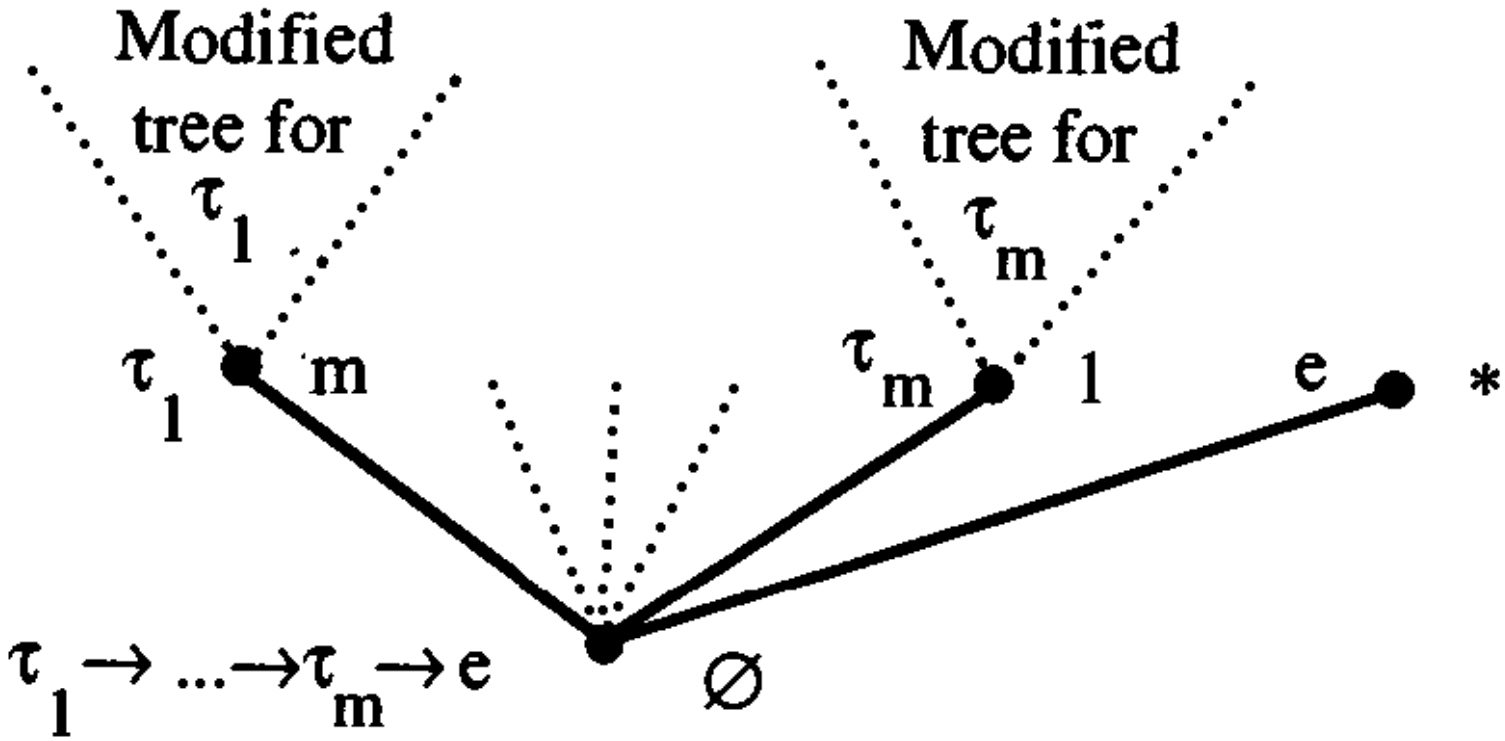
\includegraphics[scale=0.3]{fig5.png}
\end{figure}
 
\end{mydef}

\begin{mydef}[S-components] Iff a node on the condensed tree of $\tau$ is labeled with a type $\sigma$ and a position $p$ we call the triple $\langle\sigma, p,\tau\rangle$
an \textbf{s-component} of $\tau$. 
\end{mydef}

\begin{mydef}[Premises, tail] If $\rho$ is a a composite s-component of a type $\tau$ and $\rho \equiv \rho_1\,\to\,...\,\to \rho_m\,\to\,a\,\, (m \geq 1)$, the s-components
$\rho_1,\, ...,\, \rho_m$ are called the \textbf{premises} of $\rho$ and $a$ is called the \textbf{conclusion} or \textbf{tail-component} of $\rho$.
\end{mydef}


\begin{mydef}[Subpremises, subtails] An s-component of $\tau$ is called a \textbf{subpremise} of \textbf{subtail} of $\tau$ according as it is a premise or tail of another
s-component of $\tau$. The sets of all subpremises and all subtails of $\tau$ will be called, respectively,
\begin{center}
 $Subpremises(\tau),\,\,\,\,\,\,Subtail(\tau)$
\end{center}
\end{mydef}

\begin{mydef}[Positive and negative s-components] An s-component $\sigma$ of $\tau$ is called \textbf{positive} or \textbf{negative} according as the number of 
 non-asterisk symbols in tis position is even or odd. If $\sigma$ is positive we say $\sigma$ \textbf{occurs positively} in $\tau$, otherwise $\sigma$ 
 \textbf{occurs negatively} in $\tau$.
\end{mydef}
 
\begin{mydef}[$NSS(\tau)$] If $\tau$ is composite, $NSS(\tau)$ is the set of all finite sequences $\langle\sigma_1, ..., \sigma_n\rangle\,\,(n\geq 1)$ such
 that $\tau$ contains a positive s-component with form
\begin{center}
 $\sigma_1\,\to\,...\,\to\sigma_n\,\to a$
\end{center}
from some atom $a$. Each member of $NSS(\tau)$ is called a \textbf{negative subpremise-sequence} (because it is a sequence of terms that have occurrences as negative
subpremises in $\tau$).
The set of all members of the sequences in $NSS(\tau)$ will be called
\begin{center}
 $\bigcup\, NSS(\tau)$.
\end{center}
\end{mydef}


\begin{lem}[Enhanced Subformula Lemma]\label{8E7} If $Z^{\sigma}$ is a subargument of a closed long typed nf-scheme $X^{\tau}$, then
\begin{itemize}
 \item[(i)] $\sigma$ occurs as a positive subpremise in $\tau$,
 \item[(ii)] if $\tau$ is an atom, $IAT(Z^{\sigma}) = \emptyset$,
 \item[(iii)] if $\sigma$ is composite, $IAT(Z^{\sigma}) \in NSS(\tau)$,
 \item[(iv)] $NSS(\sigma) \subseteq NSS(\tau)$.
\end{itemize}
\begin{proof}
 Since $Z^{\tau}$ is long, $IAT(Z^{\tau})$ coincides with the sequence of all premises of $\sigma$, so (ii) holds. And also if $\tau$ is composite we have
 \begin{equation}\label{eq1}
  IAT(Z^{\tau}) \in NSS(\sigma)
 \end{equation}
by the definition of $NSS(\sigma)$. Now (i) implies (iv), by the lemma \textbf{9E9.2}(iii), and (iv) and (\ref{eq1}) imply (iii). Hence only (i) remains to 
be proved. 

The proof of (i) is, again, an induction in $|X^{\tau}|$. So we shall prove
\begin{quotation}
  \noindent If  $X^{\tau}$  is a long member of $\mathbb{TNS}(\Gamma)$ and  $\Gamma \equiv \{u_1:\theta_1,\, ...\, u_p:\theta_p,\,V_1:\phi_1,\,V_q:\phi_q\}$ 
  and  $Z^{\sigma}$ is a subargument of  $X^{\tau}$, then $\sigma$  occurs in a positive subpremise of 
  \begin{equation}\label{eq2}
   \theta_1\to \cdots \to \theta_p \to \tau
  \end{equation}
\end{quotation}
\begin{itemize}
 \item[(IB)] If $X^{\tau}$ is an atom the conclusion of (\ref{eq2}) holds vacuously.
 \item[(IS)] Let $X^{\tau}$ have form
 \begin{equation}
  (\lambda\,x_1^{\tau_1}\, ...\,x_m^{\tau^m}\cdot (y^{(\rho_1\to\cdots \to \rho_n\to e)}\,X_1^{\rho_1}\cdots X_n^{\rho_n})^e)^{(\tau_1\to\cdots \to\tau_m\to e)}
 \end{equation}
where $m, n \geq 0$ and $\tau \equiv \tau_1\to\cdots \tau_m\to e$. Then either $y \equiv x_i$ for some $i \leq m$ or $y \equiv u_i$ for some $i \leq p$. If $y\equiv x_i$ then
\begin{equation}
 \tau_i \equiv \rho_1\to\cdots \to \rho_n\to e
\end{equation}
and if $y \equiv u_i$ then 
\begin{equation}
 \theta_i \equiv \rho_1\to\cdots \to \rho_n\to e
\end{equation}
\end{itemize}
In both cases $\rho_1,\,...,\,\rho_n$ occurs as a positive subpremise of
\begin{equation}\label{eq3}
 \theta_1\to\cdots\to\theta_p\to\tau
\end{equation}

Now $Z^{\sigma}$ must be in an $X^{\rho_j}_j$ for some $j \leq n$. If $Z^{\sigma} \equiv X^{\rho_j}_j$ then $\sigma \equiv \rho_j$ and the conclusion of (\ref{eq2}) follows
by the above considerations. Next, suppose $Z^{\sigma}$ is a subargument of $X^{\rho_j}_j$. Note that
\begin{equation}
 X^{\rho_j}_j \in \mathbb{TNS}(\{x_1:\tau_1,\,...,\,x_m:\tau_m\}\cup\Gamma)
\end{equation}
Hence, by IH, $\sigma$ occurs as a positive subpremise of 
\begin{center}
$\tau_1\to\cdots\to\tau_m\to\theta_1\to\cdots\to\theta_p\to p_j$ 
\end{center}
Thus $\sigma$ occurs as a positive subpremise of (\ref{eq3}), given (\ref{eq2}).
\end{proof}
\end{lem}

\begin{col} 
 If $X^{\tau}$ is a closed long typed nf-scheme, the type of each meta-variable in $X^{\tau}$ either occurs as a positive subpremise of $\tau$ or is $\tau$ itself.
\begin{proof}
   Consequence of the lemmas \ref{8E2.2}(i) and \ref{8E7}(i).
 \end{proof}
\end{col}

\begin{col} If $X^{\tau}$ is a closed long typed nf-scheme and $Z^{\sigma}$ is a subargument of $X^{\tau}$ or $Z^{\sigma} \equiv X^{\tau}$, then
\begin{itemize}
 \item[(i)] $Length(IA(Z^{\sigma})) = Length(IAT(Z^{\sigma})) \leq |\tau| - 1$,
 \item[(ii)] $Length(CA(Z^{\sigma},X^{\tau})) \leq (|\tau| - 1) \times Depth(X^{\tau})$\\
 Further, if $\lambda v_1^{\rho_1}, ..., \lambda v_r^{\rho_r}$ are all the abstractors in $X^{\tau}$ (not just its initial ones), then
 \item[(iii)] $\{\rho_1, ..., \rho_r\}$ has at most $|\tau| - 1$ distinct members.
\end{itemize}
\begin{proof} Follow the proof
\begin{itemize}
 \item[For {\em (i)}:] $Length(IAT(Z^{\sigma}) \leq |\tau | - 1$ by the lemmas \ref{8E7}(iii) and \textbf{9E9.3(iv)}.
 
 \item[For {\em(ii)}:] If $Z \equiv X$ the left side of (ii) is $0$. If $Z \cancel{\equiv} X$ let $\langle Z_0,...,Z_k\rangle\,\,\,(k\geq 1)$
 be the argument branch form $X$ to $Z$; the, by the note \ref{8E5.1}(iv)
 \begin{center}
  $Length(CA(Z,X)) = Length(IA(Z_0))+\cdots + Length(IA(Z_{k-1})) \leq k(|\tau | - 1)$
 \end{center}
by (i). But $Depth(X) \geq k$ by the lemma \ref{8E4.1}(ii), so (ii) holds.
 \item[For {\em (iii)}:] Each $\rho_i$ is in $IAT(X^{\tau})$ or in $IAT(Y^{\theta})$ for subargument $Y^{\theta}$ of $X^{\tau}$; and
 in both cases $\rho_i \in \cup NSS(\tau)$ (in the former case trivially, and the later case follows by the lemmas \ref{8E7}(iii) and \textbf{9E9.3(iii)}.
\end{itemize}

\end{proof}
\end{col}


\begin{lem}[Search-Completeness Lemma]\label{8F1} Part (iii) of the theorem \ref{8C5} holds; i.e. if $\tau$ is composite and $d \geq 0$, then
\begin{center}
 $Long(\tau,d) \subseteq \mathcal{A}(\tau, \leq d + 1)$.
\end{center}

\begin{proof}
     The goal is to that $Long(\tau,d) \subseteq \mathcal{A}(\tau, \leq d +1)$ holds.
      In order to do it, a property stronger will be proved. Define
      $\mathcal{L}^*(\tau,d)$ the set of long closed nf-schemes with depth d
      such that:
      
      \begin{itemize}
             \item[(a)] All $X^{\tau}$ in $\mathcal{L}^*(\tau,d)$ is
               proper and its meta-variables have depth $d$.
             \item[(b)] All subarguments with depth $d$ in $X^{\tau}$
               are meta-variables.
      \end{itemize}
      
      The news properties to prove are:

      \begin{enumerate}
             \item $\mathcal{L}^*(\tau,d) \subseteq
               \mathcal{A}(\tau,\leq d)$
             \item $Long(\tau,d) \subseteq \mathcal{A}(\tau, \leq d +1)$
       \end{enumerate}

       The properties are proved by induction in $d$:

       \begin{itemize}
               \item[(IB)] Induction basis is $d = 0$. For property
                 {\em (a)}, there is only a nf-scheme with a depth $0$. This is
                 a meta-variable. Thus:

                 $\{V^{\tau}\}=\mathcal{L}^*(\tau,d) \subseteq
               \mathcal{A}(\tau,\leq d) = \{V^{\tau}\}$.

               For the property {\em b}, let $\tau \equiv \tau_1 \to \cdots
               \to \tau_m \to e$. Let $M^{\tau}$ a element of
               $Long(\tau,0)$. It has the form:

               $\lambda y^{\tau_1}_1 \cdots y^{\tau_m}_m \cdot
               y^{\tau_i}_i$. To construct $\mathcal{A}(\tau, 1)$, it
               outputs $\lambda y^{\tau_1}_1 \cdots y^{\tau_m}_m \cdot
               y^{\tau_i}_i$ as suitable replacement of $V^{\tau}$ in
               $\mathcal{A}(\tau,0)$, because $\tau$ is isomorphic to
               $\tau$. Hence $\mathcal{A}(\tau,1)$ must contains $\lambda y^{\tau_1}_1 \cdots y^{\tau_m}_m \cdot
               y^{\tau_i}_i$.

               \item[(IS)] Assume the properties {\em (a)} and {\em (b)} holds for $d$
                 and prove that they will hold for $d+1$. Let $X \in
                 \mathcal{L}^*(\tau,d+1)$. Then, $Depth(X) = d+1$
                 by lemma \ref{8E3.1} $X$ has a subargument whose depth in $X$
                 is $d+1$, and by lemma \ref{8E4.1} $X$ has one whose depth is
                 $d$. List all subargments: $W_1, \cdots,W_r$. 
                 Obviously, $W_1, \cdots, W_r$ are disjoint
                 components since they have the same depth $d$ in $X$.
                 Since $Depth(X) = d+1$, $Depth(W_i) \leq 1$ for each
                 $i$. $X$ satisfies {\em (a)} and {\em (b)}, so no $W_i$ is a
                 meta-variable and it must has the form:

                 $W_i \equiv \lambda x_{i,1}  \cdots {x_{i,m_i}} \cdot
                 (y_i V_{i,1} \cdots V_{i,n_i})$.

                 Let be $X`$ as a result of replace each meta-variable $V_i$
                 in $X$ by $W_i$. $X`$ is a long and closed nf-scheme
                 with depth d and it satisfies the condition {\em (b)} as a
                 member of $\mathcal{L}^*(\tau,d)$. The condition {\em (b)}
                 holds too, because if $X`$ contained a meta-variable
                 occurrence $V$ at a depth $< d$ such a $V$ could not be
                 a $V_i$ and hence would occur also in $X$ at a depth $< d$
                 contrary to the assumption that $X$ satisfies {\em (a)}
                 relative to $d+1$.

                 Hence $X` \in \mathcal{L}^*(\tau,d)$. By induction
                 hypothesis there is an $X`` \in \mathcal{A}(\tau ,\leq d)$ 
                 that is alpha equivalent to $X`$. Apply the
                 step $d+1$ of search algorithm.  It is easy to see that
                 $W_i$ is a suitable replacement for $V_i$. Hence the
                 algorithm gives $X$ as an extension of $X``$. So, $X
                 \in \mathcal{A}(\tau, \leq d+1)$ giving the property 1
                 for $d+1$.

                 In other to prove property 2, let $M \in
                 Long(\tau,d+1)$. The by \ref{8E3.1}. M has a
                 subargument whose depth in $M$ is $d+1$. List all
                 subarguments without repetitions : $U_1, \cdots,
                 U_r$. Clearly, $U_1, cdots, U_r$ are disjoints. Since
                 $Depth(M) = d+1$, each $U_i$ has depth 0. Therefore,
                 it must have the form: $U_i \equiv \lambda x_{i,1}
                 \cdots x_{i,m_i} \cdot y_i$. Let $M`$ as a
                 replacement of each meta-variable $V_i$ by $U_i$ in
                 $M$. $M`$ is a closed and long nf-scheme with depth
                 $d+1$. Also, $M`$ satisfies {\em (a)} {\em (b)} as a
                 member of $\mathcal{L}^*(\tau,d+1)$ because all its
                 meta-variables was introduced by the above
                 replacements. Hence $M` \in \mathcal{L}(\tau,d+1)$

                 Therefore by property 1, there is an $M``$, differing
                 from $M`$ only for the renaming of meta-variables
                 such that $M`` \in \leq d+1$.  Apply the step $d+1$
                 of search algorithm in $M``$. Trivially, $U_i$ is a
                 suitable replacement for $V_i$ in $M``$. Thus, the
                 algorithm outputs M as a extension of
                 $M``$. Therefore, $M \in \mathcal{A}(\tau,d+2)$.
        \end{itemize}
 
\end{proof}
\end{lem}

\begin{lem}[Detailed Stretching Lemma]\label{8F2} If $Long(\tau)$ has a member $M^{\tau}$ with depth $\geq \rVert\tau\rVert$ then
\begin{itemize}
 \item[(i)] there exists $M^{*\tau} \in Lon(\tau)$ with $Depth(M^{*\tau}) \geq Depth(M^{\tau}) + 1$,
 \item[(ii)] $Long(\tau)$ is infinite.
\end{itemize}
\begin{proof}
 {\em (ii)} follows from {\em (i)}. And to prove {\em (i)}, let $M$ a typed closed long $\beta$-nf with type $\tau$ and without variable clashes.
 Let $d = Depth(M) \geq ||\tau ||  > 1$. By the lemma \ref{8E4.1}, M has at least one argument-branch with length $d$. Choose any such branch, call it 
 \begin{equation}\label{eq4}
  \langle N_0, ..., N_d \rangle
 \end{equation}
where $N_0 \equiv M$ and $N_{i+1}$ is an argument of $N_i$, for $i = 0, ..., d - 1$. Each of $N_0, ..., N_d$ must have form
\begin{equation}
 N_i \equiv \lambda\,x_{i,1}\,...\,x_{i,m_i}\cdot y_i\,P_{i,1}\cdots P_{i,n_i}\,\,\,\,\,\,(m_i,n_i \geq 0),
\end{equation}
and for $i \leq d - 1$ we have $N_{i+1} \equiv P_{i,k_i}$ for some $k_i < n_i$ (and hence $n_i \geq 1$). Since $d = Depth(M)$
the last member (\ref{eq4}) has no arguments, so $n_d = 0$. For $i = 0, ..., d$ let $B_i$ be the body of $N_i$; that is
\begin{equation}
 B_i \equiv y_i\,P_{i,1}\cdots P_{i,n_i}
\end{equation}
Since $N_i$ is long, the type of $B_i$ is an atom. And this atom occurs in $\tau$ by the lemma \textbf{2B3(ii)}. But $||\tau || \leq d$
and there are $d + 1$ components $B_0, ..., B_d$, at least two of these must have the same type. Choose any pair $\langle p, p + r\rangle$
such that $B_p$ and $B_{p + r}$ and
\begin{center}
 $Depth(B_p) \geq r + Depth(B_{p + r})$.
\end{center}
Define $M^*$ to be the result replacing $B_{p+r}$ in $M$ by a copy of $B_p$ (after changing bound variables in this copy to avoid clashes).
Then $M^*$ has an argument-branch with length $d + r$. (Its members are 
\begin{center}
 $N_0^*, ..., N^*_{p + r}, N^o_{p + 1}, ..., N^o_d$,
\end{center}
where for $i = 0, ..., p + r$ each $N_i^*$ has the same position in $M^*$ as $N_i$ in $M$, and for $j = p + 1, ..., d$ we have $N^o_j \equiv N_j$)
hence by the lemma \ref{8E4.1},
\begin{center}
 $Depth(M^*) \geq  d + r \geq d + 1$
\end{center}
To complete the proof of {\em (i)} it only remains to show that $M^*$ is a genuine typed
term. This will be done by applying \textbf{lemma 5B2.1(ii)} on replacement in typed terms.

First, for $i = 0, ..., d$ let $\Gamma_i$ be the context that assigns to the initial abstractors of
$N_i$ i the types they have in $M$. Since $M$ has no bound-variable clashes the variables
in $\Gamma_0, ..., \Gamma_d$ are all distinct, so
\begin{equation}\label{eq5}
 \Gamma_0 \cup \cdots \cup \Gamma_d \mbox{ is consistent}.
\end{equation}
Also every variable free in $B_i$ B; is bound in one of $N_0, ..., N_i$ because $M$ is closed and $B_i$ is in $N_i$.
Hence, by the definitions of typed term \textbf{(5A1)} and $Con$ \textbf{(5A4)},
\begin{equation}\label{eq6}
 B_i \in \mathbb{TT}(\Gamma_0 \cup \cdots \cup \Gamma_i), \,\,\,\,\,\,\, Con(B_i) \subseteq \Gamma_0 \cup \cdots \cup \Gamma_i
\end{equation}
To apply \textbf{5B2.1(ii)} it is enough to show that the set
\begin{equation}\label{eq7}
 Con(B_p)\cup Con(M)\cup\Gamma_0\cup \cdots \cup \Gamma_{p + r}
\end{equation}
is consistent. (The abstractors in $M$ whose scopes contain $B_{p + r}$  are exactly the initial
abstractors of $N_0, ..., N_{p + r}$). But $M$ is closed, so $Con(M) \equiv \emptyset$. And by (\ref{eq6}),
\begin{center}
 $Con(B_p) \subseteq \Gamma_0 \cup \cdots \cup \Gamma_p \subseteq \Gamma_0 \cup \cdots \cup \Gamma_{p + r}$.
\end{center}
Then (\ref{eq7}) is consistent by (\ref{eq5}).
\end{proof}
\end{lem}


\begin{lem}[Detailed Shrinking Lemma]\label{8F3} If $Long(\tau)$ has a member $M^{\tau}$ with depth $\geq \mathbb{D}(\tau)$ then
 \begin{itemize}
  \item[(i)] it has a member $M^{*\tau}$ with
  \begin{center}
    $Depth(M^{\tau}) - \rVert\tau\rVert \leq Depth(M^{*\tau}) < Depth(M^{\tau})$,
  \end{center}
  \item[(ii)] it has a member $N^{\tau}$ with
  \begin{center}
   $\mathbb{D}(\tau) - \rVert\tau\rVert \leq Depth(N^{\tau}) < \mathbb{D}(\tau)$
  \end{center}
 \end{itemize}
\begin{proof}
 Part {\em (ii)} is proved by repeating {\em (i)} and taking the first output with depth $< \mathbb{D}(\tau)$.

 Part {\em (i)} is proved as follows. Let $M$ be member of $Long(\tau)$ without bound-variable clashes.
 Let $d = Depth(M) \geq \mathbb{D}(\tau)$. In fact $\mathbb{D}(\tau) \geq 2$ because $\tau$ is composite e since atomic types have no inhabitants.

 By the lemma \ref{8E4.1}, $M$ has at least one argument-branch with length $d$; to reduce the depth of $M$
 we must shrink all these branches. Consider any such branch; just as in the proof of the stretching lemma \ref{8F2} it has form
\begin{equation}\label{eq8}
  \langle N_0, ..., N_d \rangle
 \end{equation}
where $N_0 \equiv M$ and $N_{i+1}$ is an argument of $N_i$, for $i = 0, ..., d - 1$. And
\begin{equation}\label{eq9}
 N_i \equiv \lambda\,x_{i,1}\,...\,x_{i,m_i}\cdot y_i\,P_{i,1}\cdots P_{i,n_i}\,\,\,\,\,\,(m_i,n_i \geq 0),
\end{equation}
and for $0 \leq i \leq d - 1$. Let the type of $N_i$ be
\begin{equation}\label{eq10}
 \rho_i \equiv \rho_{i,1} \to \cdots \to \rho_{i,m_i} \to a_i . 
\end{equation}
 Then since $N_i$ is long, types of $x_{i,1}, x_{i,2}, ...$ are exactly $\rho_{i,1}, \rho_{i,2}, ...$; i.e.
\begin{center}
 $IAT(N_i) = \langle \rho_{i,1}, ...,  \rho_{i,m_i} \rangle$.
\end{center}
Just as in the proof of the lemma \ref{8F2} let $B_i$ the body of $N_i$ for $i = 0, ..., d$. Then the type of $B_i$
is the tail of the type $N_i$, namely $a_i$.

Define a sequence of integers $d_0, d_1, ...$ thus $d_0 = 0$ and $d_{j+1}$ is the least $i > d_j$ such that $IAT(N_i)$
differs from all of
\begin{equation}\label{eq11}
 IAT(N_{d_0}), IAT(N_{d_1}), ..., IAT(N_{d_j}).
\end{equation}
Let $n$ be the greatest integer such that $d_n$ is defined. The branch (\ref{eq8}) has only $d$ members after $N_0$, 
so $n \leq d$ and $d_n \leq d$. Then
\begin{equation}\label{eq12}
 0 = d_0 < d_1 < \cdots < d_n \leq d.
\end{equation}
and for $0 \leq i \leq d$, $IAT(N_i)$ is identical to one of
\begin{equation}\label{eq13}
 IAT(N_{d_0}), IAT(N_{d_1}), ..., IAT(N_{d_n}).
\end{equation}
Also the $n+1 \,IAT$'s in (\ref{eq13}) are distinct, and by the lemma \ref{8E7} they are either empty or members of $NSS(\tau)$.
Hence by \textbf{9E9.3(ii)},
\begin{equation}\label{eq14}
 n + 1 \leq |\tau|.
\end{equation}
Now $d_0, ..., d_n$ partition the set $\{0, 1, ..., d\}$ into the following $n + 1$ non-empty sets which will be called
\textbf{\em IAT-intervals}:
\begin{center}
$
\begin{array}{lllll}
\mathbb{I}_j & = & \{d_j, d_j + 1, ...,  d_{j + 1} - 1\} & & (0 \leq j \leq n - 1)\\
\mathbb{I}_n & = & \{d_n, d_n + 1, ..., d\} .\\
\end{array}
$
\end{center}
If $\mathbb{I}_j$  contains two numbers $p$, $p + r$ such that $r \geq 1$ and $B_p$  and $B_{p + r}$ have the same type
(i.e. $a_p \equiv a_{p+r}$) we shall call $\langle p, p + r\rangle$ a \textbf{\em tail-repetition}. It will be called
\textbf{\em minimal} iff there is no other tail-repetition $\langle p', q'\rangle$ with 
\begin{center}
 $p \leq p' < q' \leq p + r$ 
\end{center}
Now an $\mathbb{I}_j$ that contains no tail-repetitions must have $\leq ||\tau||$ members. Because for such an $\mathbb{I}_j$ the atoms
\begin{center}
 $a_{d_j}, ..., a_{d_{j+i-1}}$
\end{center}
must all be distinct, and by (\ref{eq10}), each $a_i$ occurs in $\rho_i$, which occurs in $\tau$ by the lemma \ref{8E7}, and 
there are only $||\tau||$ distinct atoms in $\tau$. This argument also shows that for a minimal tail-repetition 
$\langle p, p + r\rangle$ we have 
\begin{equation}\label{eq15}
 r \leq ||\tau||
\end{equation}
Now there are $n + 1$ IAT-intervals in the given branch and $n + 1 \leq ||\tau||$ by (\ref{eq14}), so if
no interval contained a tail-repetition the branch would have $\leq |\tau| \times ||\tau||$ members.
But the branch has $d + 1$ members and
\begin{center}
 $d + 1 = Depth(M) + 1 \geq \mathbb{D}(\tau) + 1 >  |\tau| \times ||\tau||$ 
\end{center}
Hence at least one IAT-interval contains a tail-repetition.

We start to build $M^*$  as follows. In the given branch take the last $\mathbb{I}_j$ containing a tail repetition,
choose a minimal tail-repetition $\langle p, p + r\rangle$ in it, and change $M$ to a new term $M'$ by replacing $B_p$ by $B_{p + r}$.

To see that $M'$ is a genuine typed term we apply \textbf{5B2.1(ii)} similarly to the proof
of the lemma \ref{8F2}. Using the notation of (\ref{eq11}) in that proof, it is enough to show that the set
\begin{equation}\label{eq16}
 Con(B_{p+r})\cup Con(M)\cup\Gamma_0\cup\cdots\cup\Gamma_p
\end{equation}
is consistent. But, as in the proof of the lemma \ref{8F2}, $Con(M) = 0$ and $Con(B_{p+r})$ is a subset of
$\Gamma_0\cup\cdots\cup\Gamma_{p + r}$, so (\ref{eq16}) is consistent by (\ref{eq11}) in the proof of the lemma \ref{8F2}.

It is straightforward to prove that $M'$ is a long $\beta$-nf with the same type as $M$.
Also that $|M'| < |M|$.

But $M'$ might not be closed, because the change from $M$ to $M'$ has removed the
initial abstractors of $N_{p+1},...,N_{p+r}$ from $M$, and so some free variable-occurrences
in $B_{p+r}$ that were bound in $M$ might now be free in $M'$. To close $M'$, apply the
following procedure to every such variable-occurrence.

Let $v$ be free in the occurrence of $B_{p+r}$ in $M'$ that has replaced $B_P$ in $M$, and let $v$
be also free in $M'$. Then $v$ does not occur in a covering abstractor of this occurrence
of $B_{p+r}$ in $M$. But these covering abstractors are exactly the initial abstractors of
$N_0, ..., N_P$ in $M$, so
\begin{center}
 $v \notin IA(N_0)\cup\cdots\cup IA(N_p)$
\end{center}

But $M$ is closed, so the free $v$ in $B_{p+r}$ in $M$ must be in the scope of a $\lambda v$ in one of
$IA(N_0), ..., IA(N_{p+r})$. Hence $v$ occurs in $IA(N_h)$ for some $h$ with $p + 1 < h < p + r$;
in the notation of (\ref{eq9}) we have
\begin{center}
 $v \equiv x_{h, k}$
\end{center}
for some $k < m_h$. And the type of $v$ is $\rho_{h,k} \in IAT(N_h)$. Now by the definition of
$d_0, ..., d_n$ and the fact that the tail-repetition $\langle p, p + r\rangle$ we are eliminating is in an
interval $\mathbb{I}_j$, $IAT(N_h$) coincides with one of
\begin{center}
 $IAT(N_{d_0}),..., IAT(N_{d_j})$;
\end{center}
say $IAT(N_h) = IAT(N_{d_q})$ for some $q \leq j$. Hence there is a variable
\begin{center}
 $x_{d_q,k} \in IA(N_{d_q})$
\end{center}
with the same type as $v$. Replace $v$ by this variable throughout $M'$. The result will
be a long $\beta$-nf with the same type and depth as $M'$ and containing one less free
variable.

Similarly replace every variable of $B_{p + r}$, that is free in $M'$ by a new one which has
the same type but is bound in $M'$. The result will be a long $\beta$-nf M" with the same
type and depth as $M'$ and which is closed.

Now $M"$ has been obtained by removing a type-repetition from an argument-branch in 
$M$ which originally contained $d$ subarguments. And by (\ref{eq15}) the number of
subarguments removed is $< ||\tau||$. Hence
\begin{equation}\label{eq17}
  d - ||\tau|| \leq Depth(M") \leq d.
\end{equation}

If $Depth(M") < d$; define $M* \equiv M"$. If not, select a branch in $M"$ with length
$d$ and apply the above removal procedure to it, then continue shortening branches
with length $d$ until there are none left. (This process must terminate because each
removal strictly reduces $|M|$.) Define $M*$ to be the first term produced by this
procedure whose depth is less than $d$. Then
\begin{center}
 $d - ||\tau|| \leq Depth(M*) < d$
\end{center}
as required.

\end{proof} 
\end{lem}

\section{Conclusion}

The presented search and count algorithms are efficient to showing which are the 
normal inhabitants of a given type $\tau$. But other often problems isn't reached: 
\begin{itemize}
 \item [(i)] Counting principal normal inhabitants ($Nprinc(\tau)$, $Nprinc_{\eta}(\tau)$) or counting principal inhabitants in general ($Princ(\tau)$). 
 As discussed in the remark \ref{8A13}, there are some types $\tau$ that have the following property: 
 given $M_1^{\tau}, M_2^{\tau}$ we have that $M_1$ is a $\beta$-normal inhabitant but not principal, and $M_2^{\tau}$ is a principal but not $\beta$-normal.
 Characterize in general this class of types is a open problem;
 \item [(iii)] Counting inhabitants in a restricted classes of terms, for example the $\lambda I$-terms,
BCK$\lambda$-terms or BCI$\lambda$-terms is not a trivial problem, and the proof of the crucial shrinking lemma (lemma \ref{8D3}) would need a reformulation for each class.
\end{itemize}

Moreover, at the first glance, the complexity of the count algorithm seems to be $\mathbb{D}(\tau) = |\tau| \times ||\tau||$, but it is not correct.
Each step call for listing a set $\mathcal{A}(\tau, d)$, and this list can be large. In fact the equivalent problem that is deciding whether $\tau$ are probable in Intuitionist 
Implicational Logic is known as polynomial-space complete problem.

\end{document}
